\chapter{Background and Overview of End to End Modeling Methods}

\section{Chapter Abstract}

This chapter presents the methods used to identify the scope of this dissertation's research for the total costs of ownership of data centers. These are the methods used to understand and address the scope of research questions that seek to address total costs of building infrastructure of hyper-scale internet data centers. It begins by describing data centers based on past literature to set the context of the research undertaking. Then the chapter presents the resulting modeling framework from the culmination of the literature reviews and the researcher's professional experiences. The framework proven to be capable of quantifying the end to end costs of a global system using life cycle analysis methods by demonstrating its effectiveness with the quantification of $CO_2$ emissions. 

\section{Introduction}

    This research considers energy and $CO_2$ inventories across the life time of hyper-scale data centers (DC). These DCs house scalable computational architectures consisting of buildings, cooling plants, power distribution systems, compute hardware, digital storage hardware, and network hardware which are the status-quo for internet service operations. Physically, the size of individual internet DC facilities have increased from modest footprints to now span millions of square feet over the last decade; coinciding with ubiquitous penetration of the internet into the lives of people around the world . The increase in demand for DCs motivates this work as a tool kit in the DC building infrastructure design process. Beyond, the building design process, this kit is intended to be an element for broader business models for internet products.
    
    For internet products, DCs represent a major fraction of their total costs of operations and environmental footprints.  This work develops a modeling framework that couples building energy models, marginal cost of grid energy models, and the embodied costs of materials to provide an end to end assessment of data centers. Specifically, this dissertation demonstrates the models by quantifying the $CO_2$ emissions as a singular metric that is is sufficiently analogous monetary costs.
    
    In the next section, some background and past literature about the sustainability of data centers is presented first. The background indicates the research motivation behind the life cycle perspective for data center systems. Then second, seminal works that have analyzed data center life cycle costs are reviewed. These works guide the development of resulting model from this research by pointing to low hanging fruits and gaps in the current practices. Then third, details about data center infrastructure is provided that 

\section{Background}

    Data centers (DCs) will consume 13\% of the worlds energy production by 2030 according to worst case prediction models \cite{andrae15}. This high energy demand is not surprising given the ubiquitous penetration of the internet nowadays. For internet DC infrastructure, the energy demand problem space is compounded by a rapid pace of hardware technology innovations on one hand. On the other hand, factoring software technology innovations lead to models that show a brighter picture. This picture is aligned with current trends, where efficiency across the entire DC stack indicates a downward trend for power demand per unit of performance. As an example, by 2016 performance throughput had increased 350\% since 2012, relative to the power demand for computer hardware \cite{GoogleEnvRpt}.  The hardware efficiency gains seen over the last decade still do not offset the need for additional DC physical capacity.
    
    Internet DC capacity is not bound by physical sizes or geographic locations however. Location agnostic networks spanning the globe allow information technology (IT) systems to scale in resource parameters such as CPU, GPU, memory, storage, and data access rates. Parametric scaling of these resources enables operational tuning to compensate for physical capacity constraints. Capacity fungibility of DC parameters at a global scale leads businesses with risky practices to provision building scale data-center infrastructure very lean. While businesses that are adverse to risk can be excessively conservative. In the case of lean provisioning, all physical resources are highly utilized with little or no headroom. For the conservative approaches, normal operating conditions are such that sustained operational points are well below the capacity of the equipment. Operations significantly below capacity allows the service to accept bursts in service, inorganic  growth, and be fault tolerant in case of failures elsewhere in the system. 
    
    Lean and conservative operations are both classified as equivalent based on today's sustainability indicators and both have strategic advantages for data center owners. For example the abrupt change in internet traffic for many communications, media, and collaboration web sites due to COVID have critical dependencies on data center facilities. These change in traffic pattern are shown in Figure~\ref{img_nyt_covid}, if the data centers were operational loaded to peak capacity then it would be impossible to absorb such drastic changes.
    
    \begin{figure} [!h]
\centering
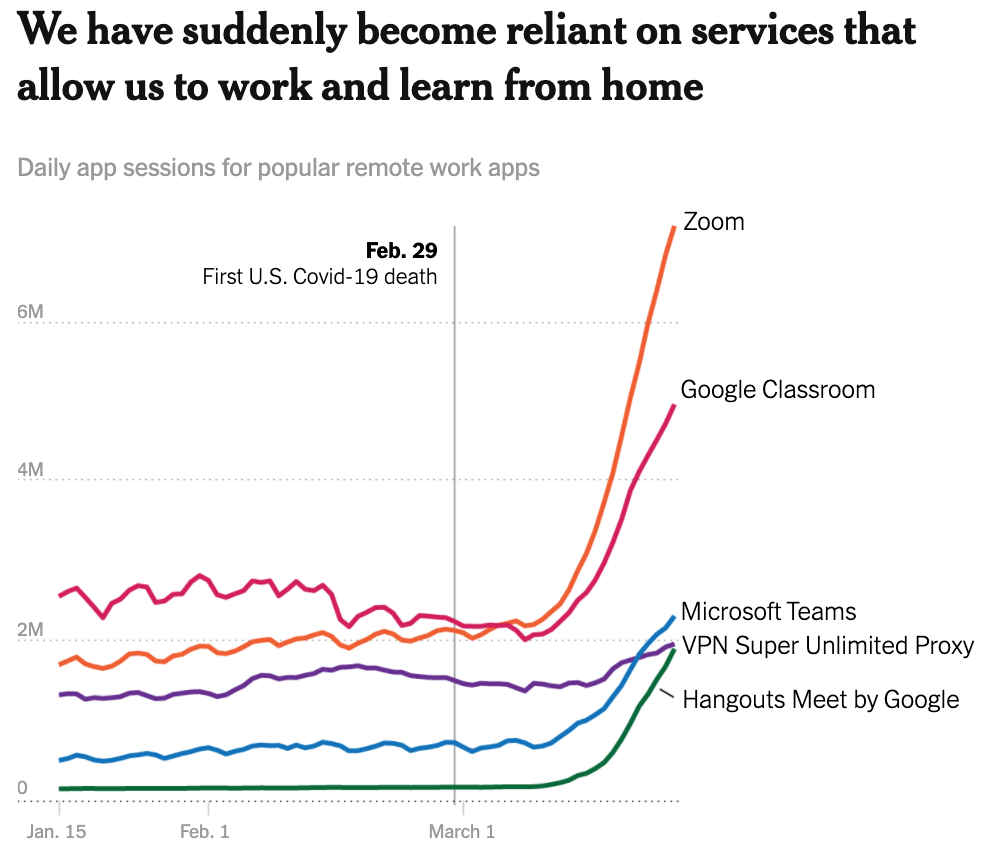
\includegraphics[scale=.3]{methodology/images/nyt_covid_internet.png}
\caption[Internet Traffic Change due to COVID]{Internet Traffic Change.  Image from \cite{nyt_corna_virus}}
\label{img_nyt_covid}
\end{figure}
    
    Furthermore, DC facilities can be measured with multiple attributes; power limits, cooling limits, network limits, and floor space. Where power has shown to be the most prevalent indicator of DC, \cite{barroso18}. However, the other attributes don't linearly scale with power. For example, the researcher designed a data center in mid 2013 based on historical trends. By the time the data center was deployment the power density per information technology devices had significantly increased. With the increase in the power density, more that 60\% of the designed floor space was left stranded (ie not deploy-able as the facility was power and cooling limited at 40\% of the designed area). However, if the DC design team had looked closer at Moore's law such disruptive change in density were apparent. Figure~\ref{img_moores} indicates the log-scale nature of de-materialization of transistor based technology made famous by Moore.
    
    \begin{figure} [!h]
\centering
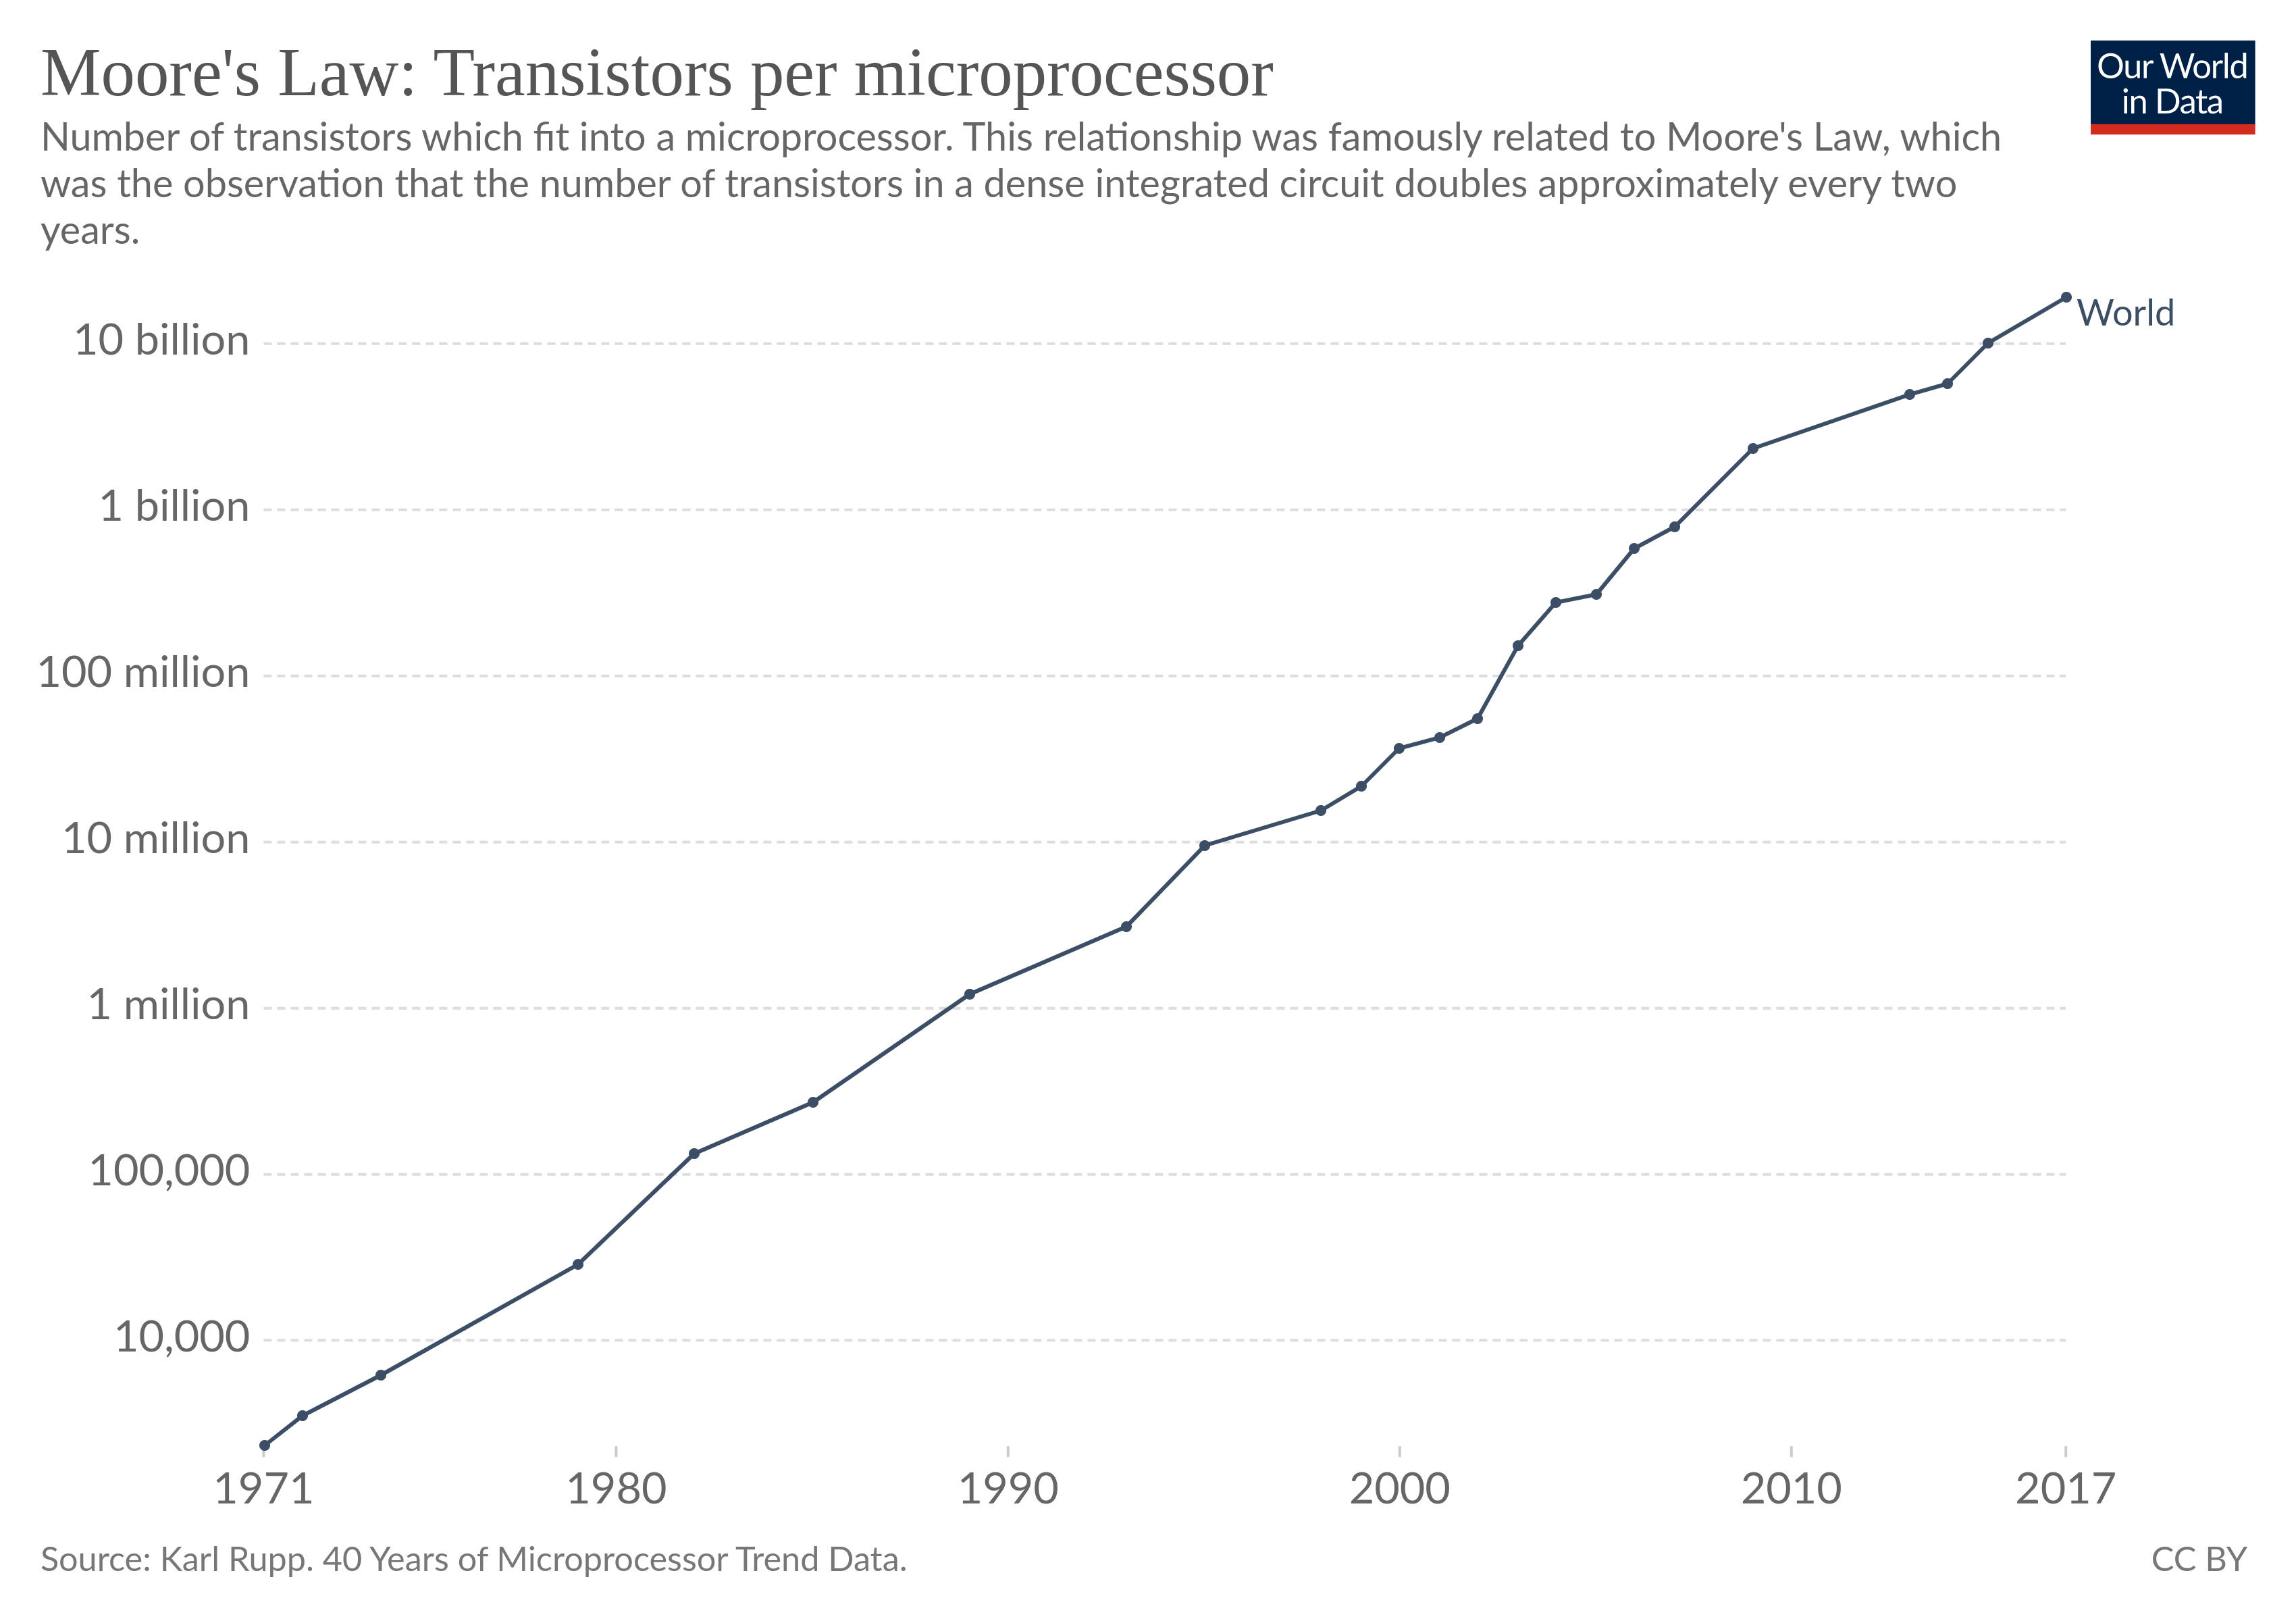
\includegraphics[scale=.1]{methodology/images/transistors-per-microprocessor.png}
\caption[Moore's Law]{Moore's Law: Transistors per microprocessor.  Image from \cite{world_data}}
\label{img_moores}
\end{figure}
    
    The prevalent indicator for sustainability of DC facilities is currently the Power Usage Effectiveness metric ($PUE$, see equation \ref{eq:pue}). $PUE$ is a dimensionless ratio of load vs. supply energy.   In the equation $E_{IT}$ indicates the IT energy load and $E_{total}$ indicates the total energy supplied to the facility. The $PUE$ is generally reported in a quarterly or annual basis by integrating the equation across the respective time period. For a given period, the metric measures the operational efficiency of the facility's system compared to the information technology equipment (ITE). Spaces housing ITE have seen profound cooling and power distribution efficiency gains resulting from the focus on $PUE$, however the metric does not comprehensively cover sustainability of DCs.
    
        \begin{equation} \label{eq:pue}
    PUE=\frac{E_{total}}{E_{IT}} 
    \end{equation}
    \begin{center}
    $E_{total}$ = Total Power Used at Facility
    
    $E_{IT}$ = Power Consumed by IT Equipment
    \end{center}
    \vspace{.2cm}
    
    
    The $PUE$'s shortcomings as a sustainability metric are noted by Horner, particularly that low PUEs do not correlate to low carbon footprint \cite{Horner16a}. The tendency of carbon intensity to vary based on energy source characteristics is demonstrated by Masanet in \cite{Masanet13a}. Masanet shows that energy supply sources must be coupled with lowered demands to be good indicators of use phase carbon footprint. For example, the carbon footprint of a low $PUE$ DC with it's energy sourced from a coal plant will be higher compared to a DC that operates with a slightly higher $PUE$ but sources power from a renewable source. This is summarized in Figure~\ref{masanet13a1}.
    
    \begin{figure} [!h]
\centering
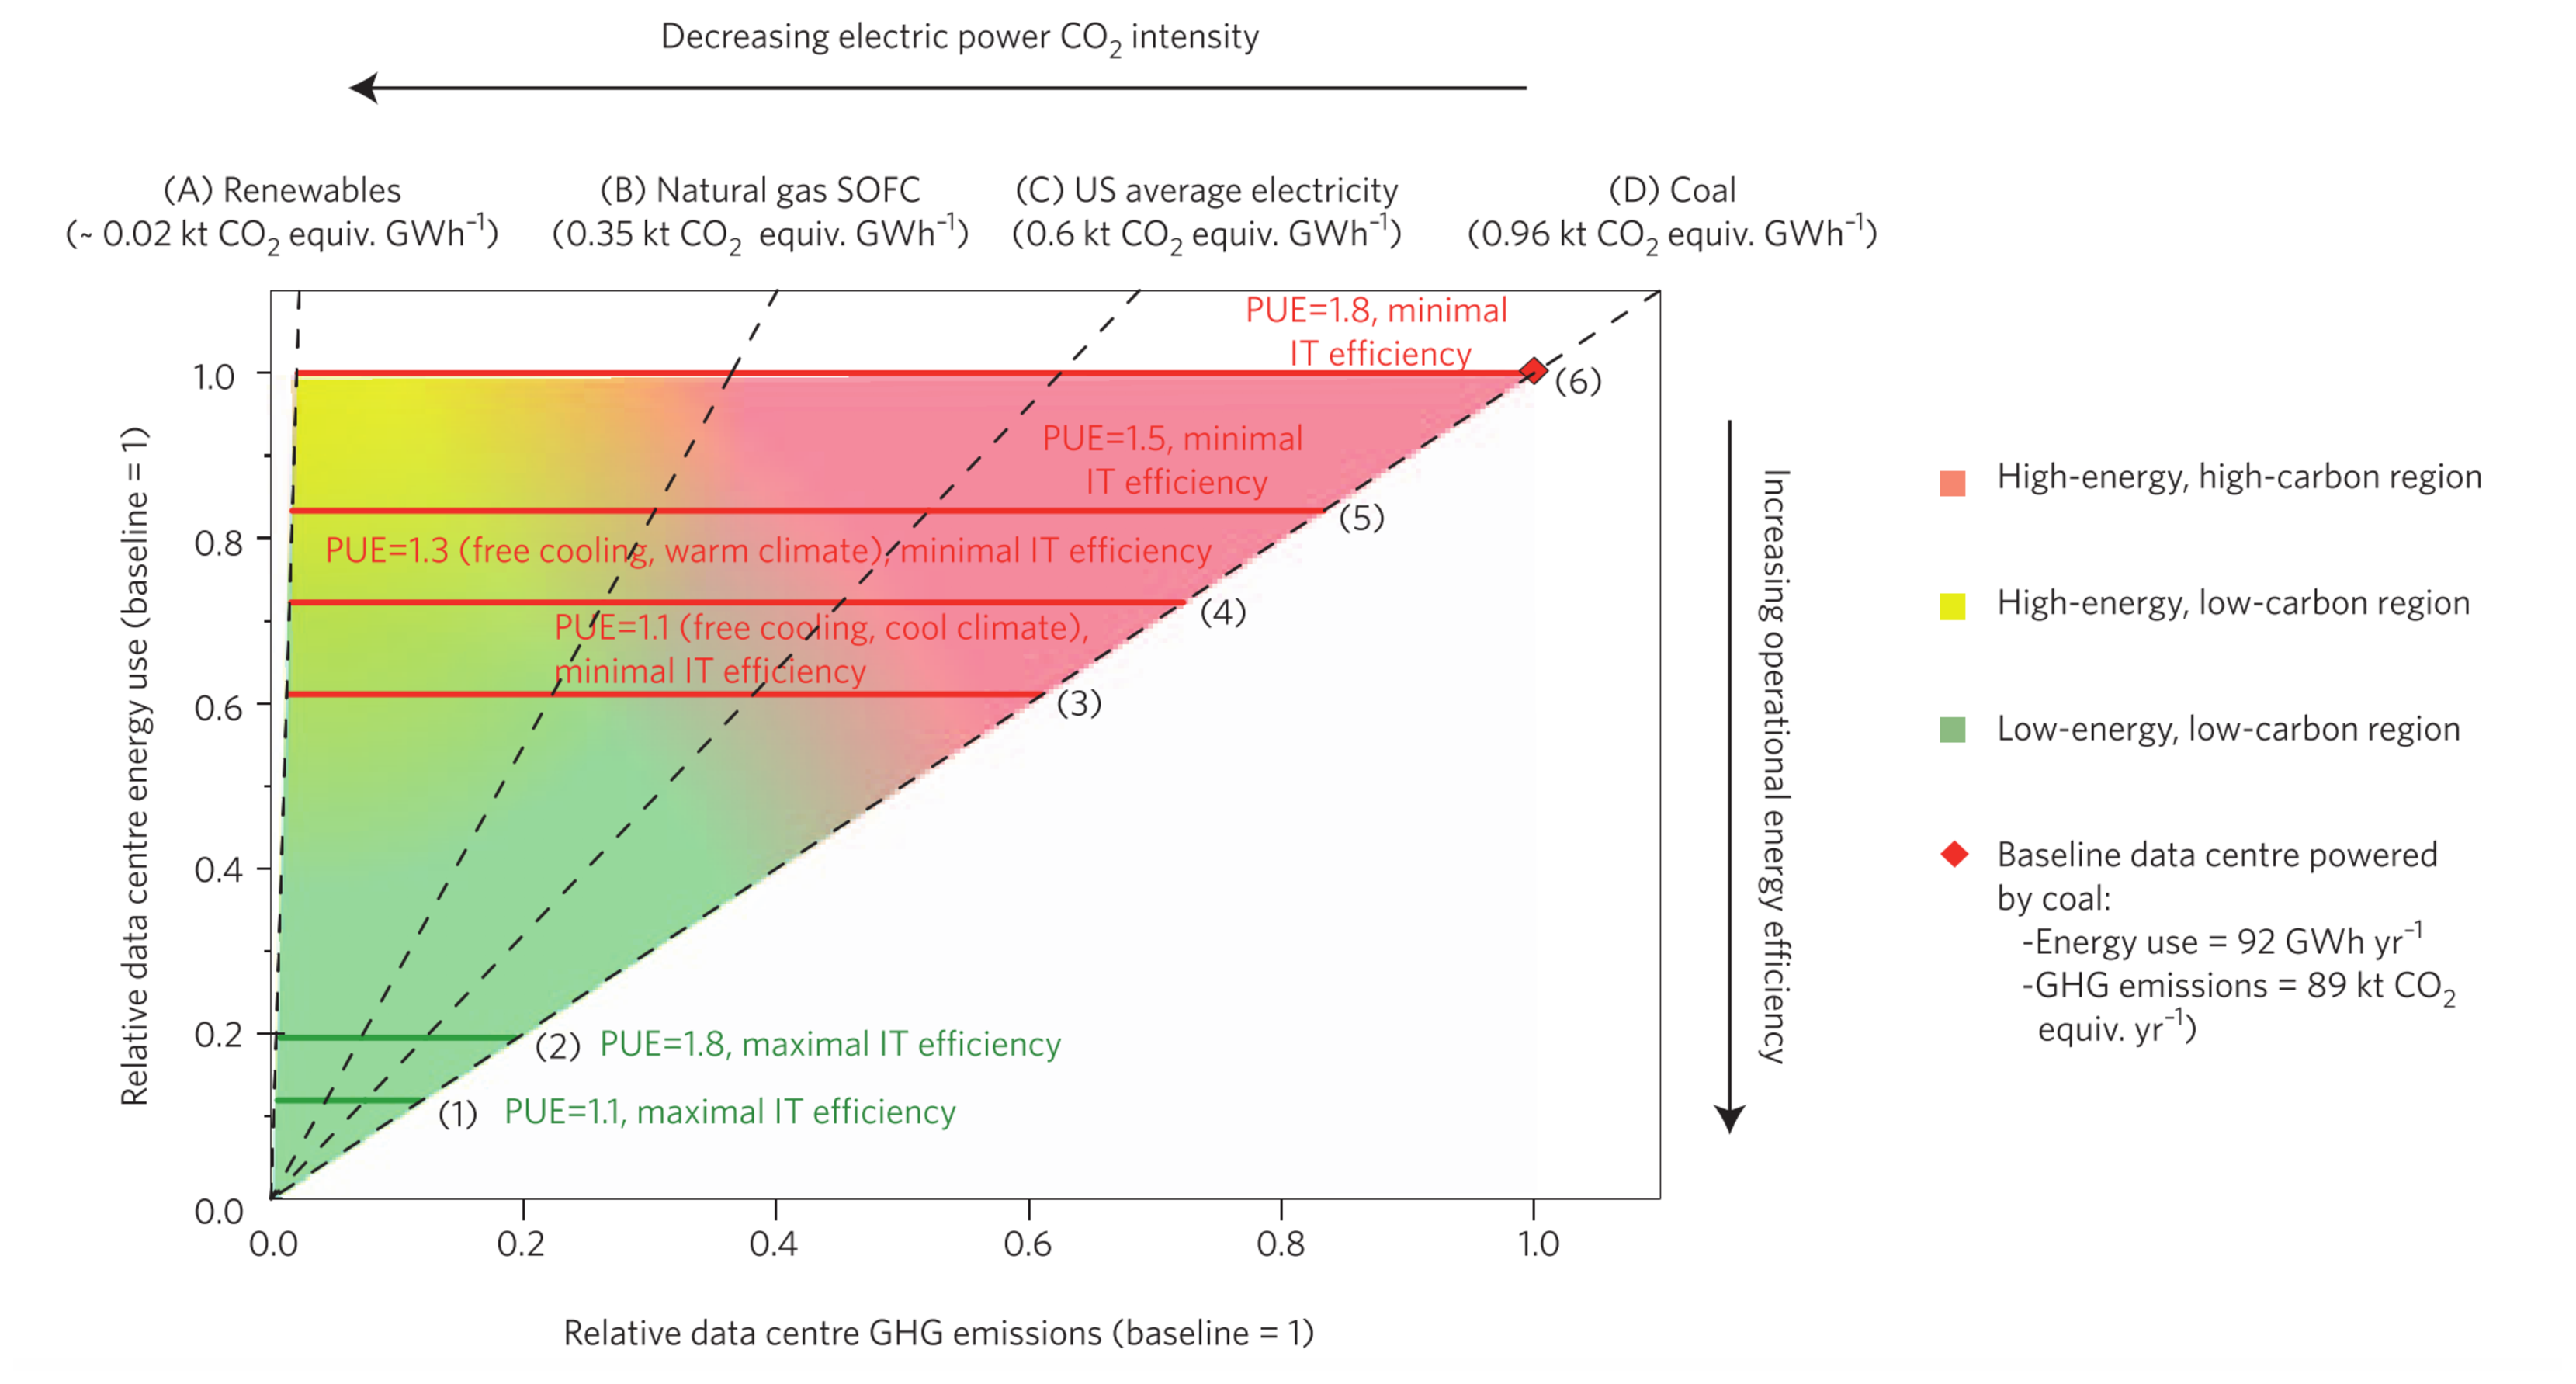
\includegraphics[scale=.25]{methodology/images/masanet13a1.eps}
\caption[Energy Use vs. Carbon performance map]{Energy Use vs. Carbon performance map. Image from \cite{Masanet13a}}
\label{masanet13a1}
\end{figure}
    
    With the proliferation of the PUE as the de-facto efficiency metric, ASHRAE recognized the significance of the cooling systems to the data center energy use. In rapid response they began to develop guidelines to help operators optimize their cooling systems. One of the most profound contribution from ASHRAE has been their position on expanded thermal window for the data center environments. The expanded thermal window has an influence nearly all elements of a data center facility. 
    
    \begin{figure} [!h]
\centering
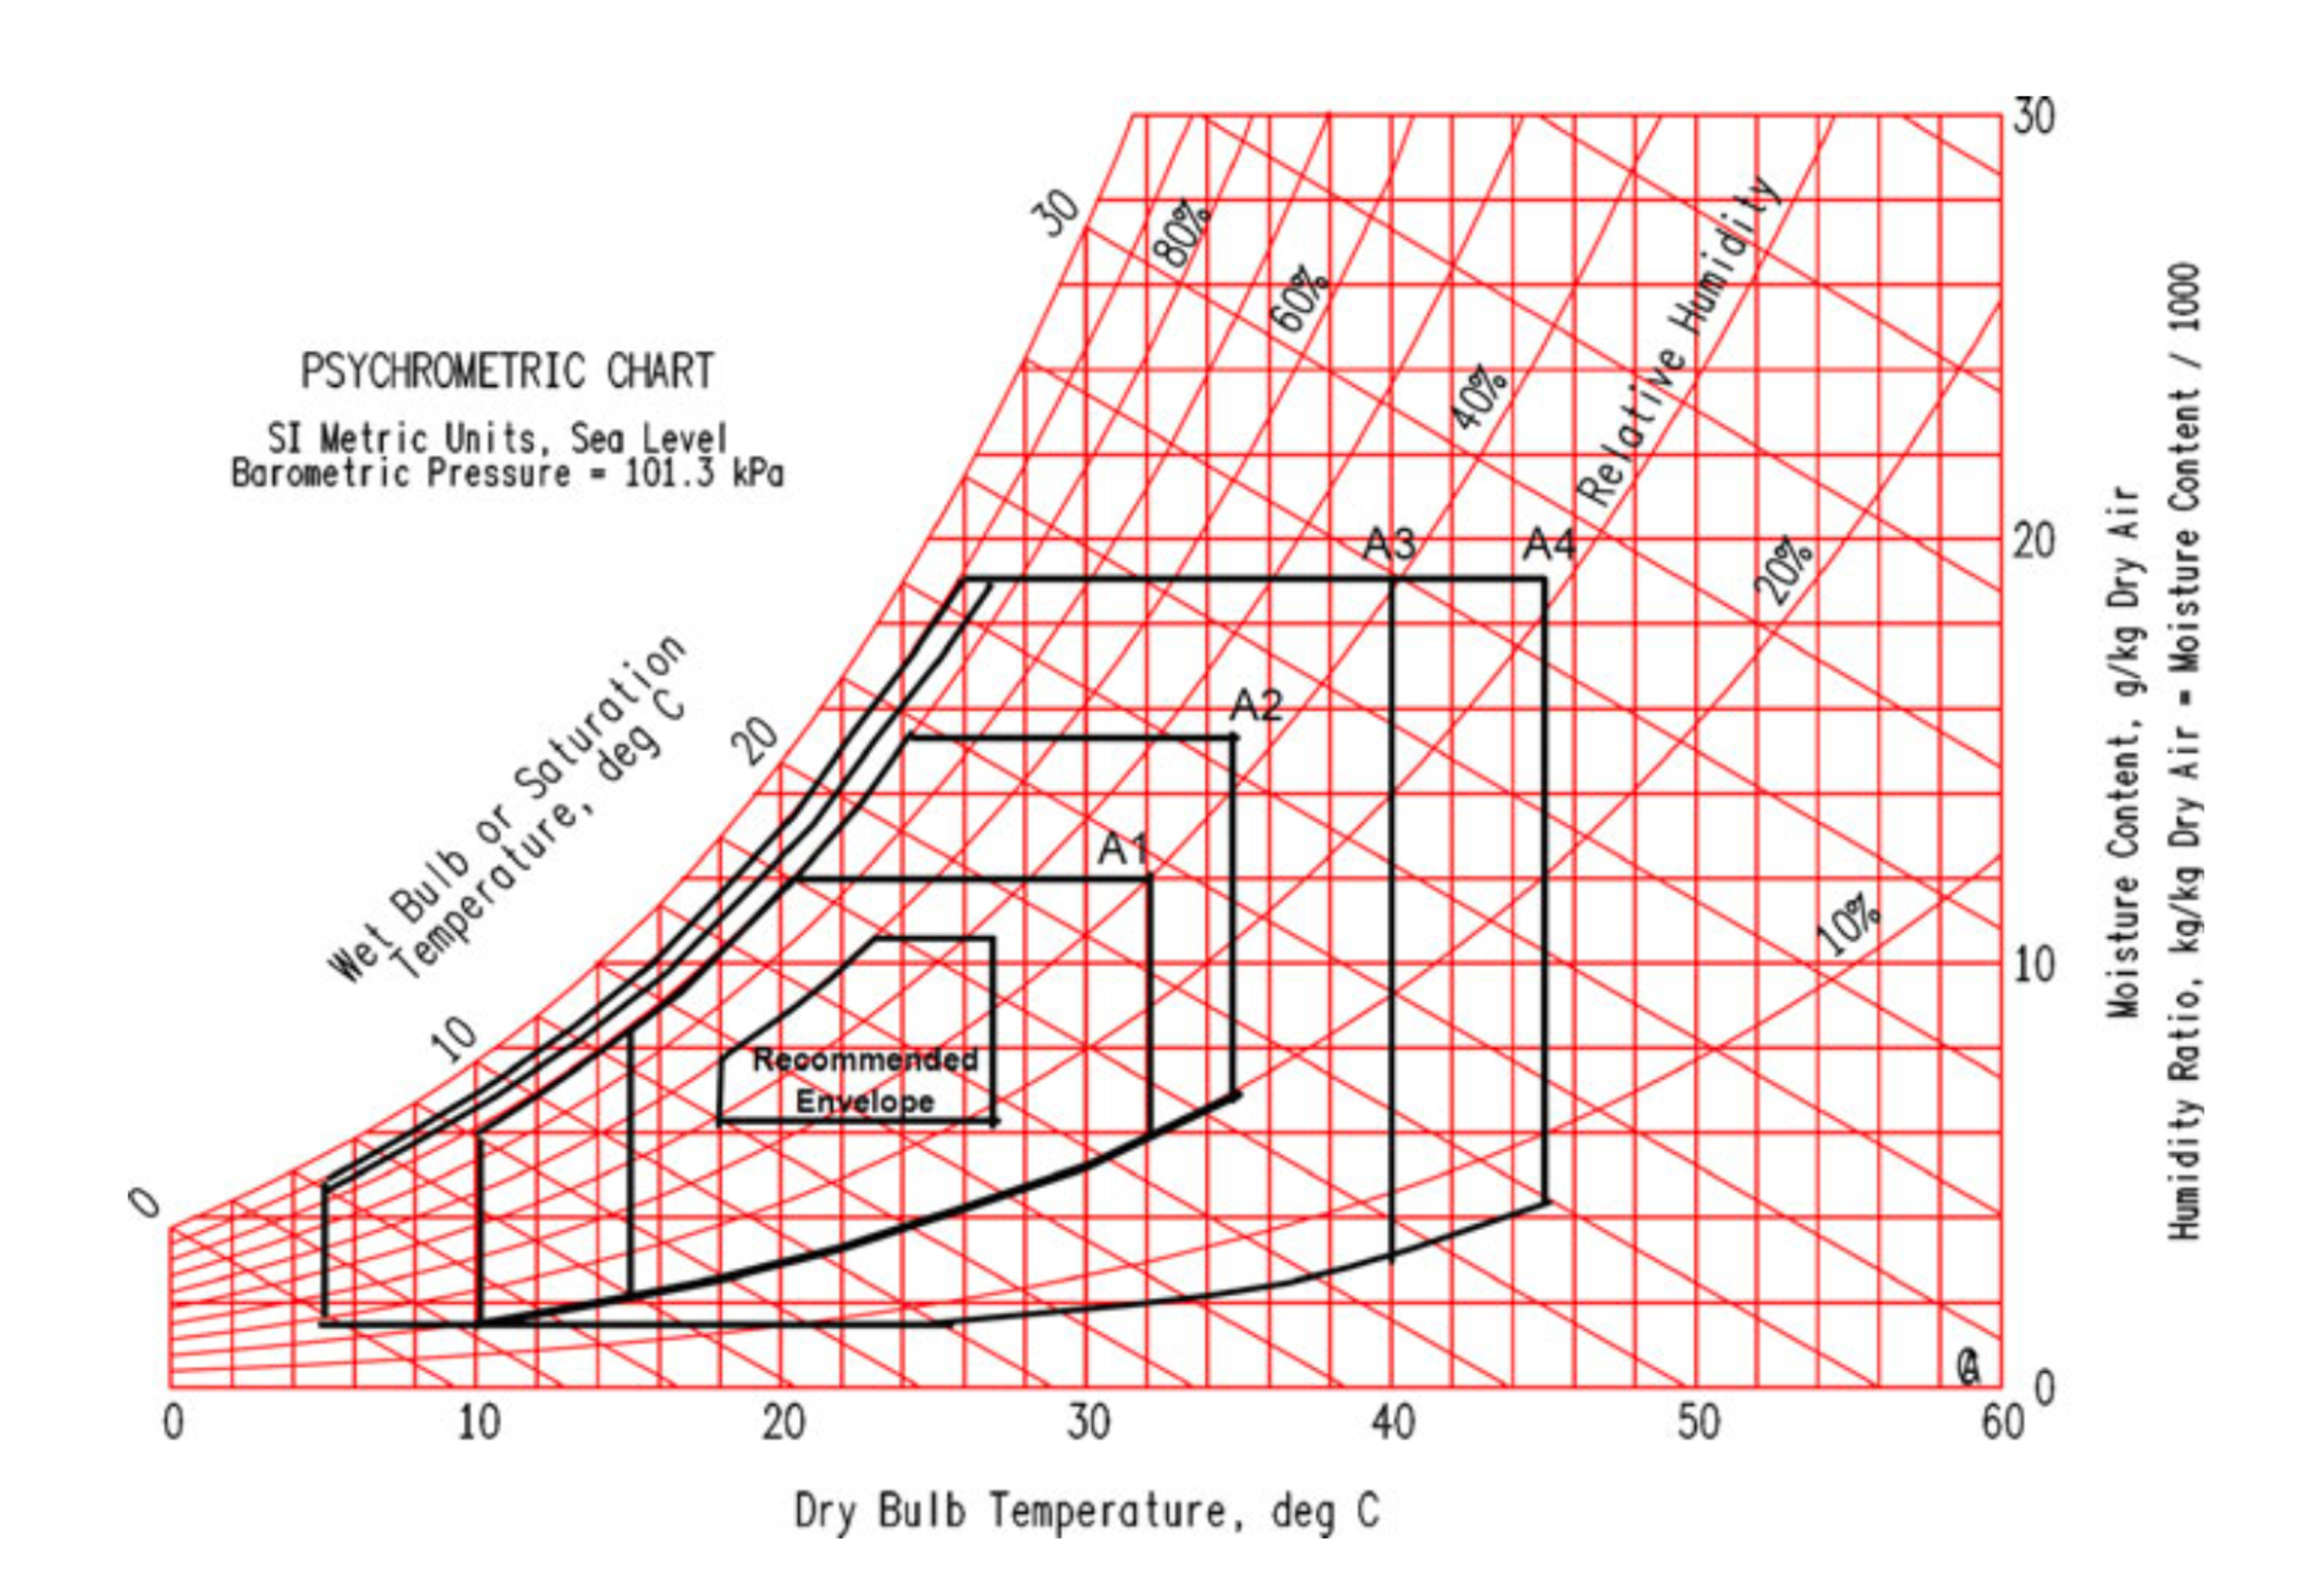
\includegraphics[scale=.3]{methodology/images/psychrometric.eps}
\caption[ASHRAE thermal environment envelope]{ASHRAE thermal environment envelope. Inlet air temperature of IT equipment (\textcopyright 2011 ASHRAE).  Image from \cite{joshi12}}
\label{psychrometric}
\end{figure}
    
    A facility's thermal environment is directly couples the IT and building systems. The first order impacts of this coupling are on the cooling system; spanning from the cooling tower to the node junctions on the nano-scale transistor junctions. The end to end flow of the heat rejection is shown in Figure~\ref{img_dc_infrastructure}. 
    
    \begin{figure} [!h]
\centering
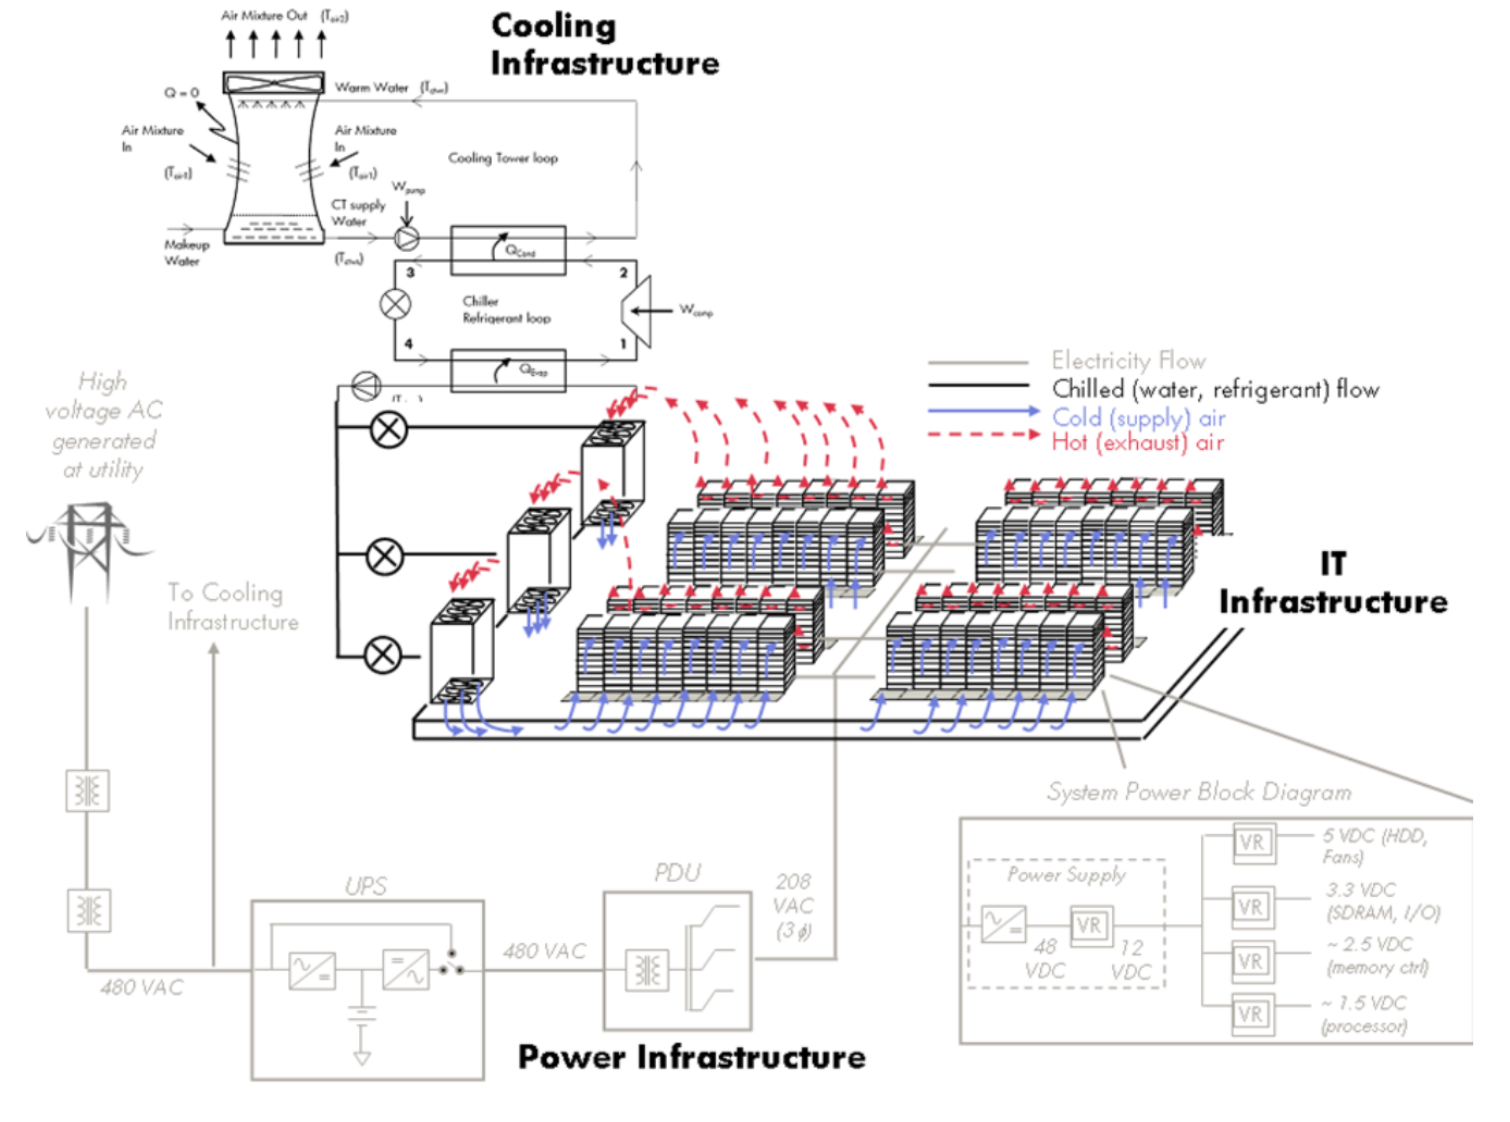
\includegraphics[scale=.25]{methodology/images/dc_cooling.png}
\caption[Image of DC heat rejection paths]{DC Infrastructure Heat Rejection Paths. Image from \cite{shah11}}
\label{img_dc_infrastructure}
\end{figure}
    
    However, there are many second order effects that must me taken into account when developing disruptive designs. The researcher's need for a life cycle analysis framework was recognized during the development of a novel bottom-cooled hermetic rack \cite{gao16}. The test chamber for the cooling coil and the computational fluid dynamic model of the bottom-cooled rack is shown in \ref{bcu_bench} and \ref{bcu_rack}, respectively. This development alone required a deep trade-off analysis of various systems that could most appropriate be done with a life cycle analysis framework. 
    
    \begin{figure}[!tbp]
    \subfloat[BCU Air Flow Chamber]{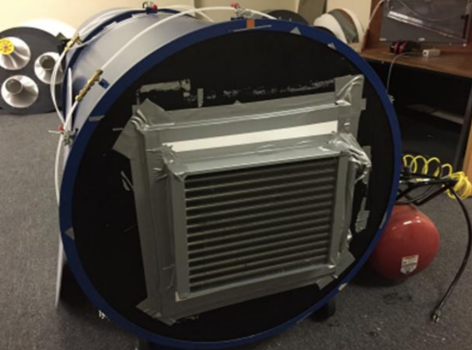
\includegraphics[width=0.35\textwidth]{methodology/images/bcu_airflow_bench.png}
        \label{bcu_bench}}
    \hfill
    \subfloat[BCU Rack]{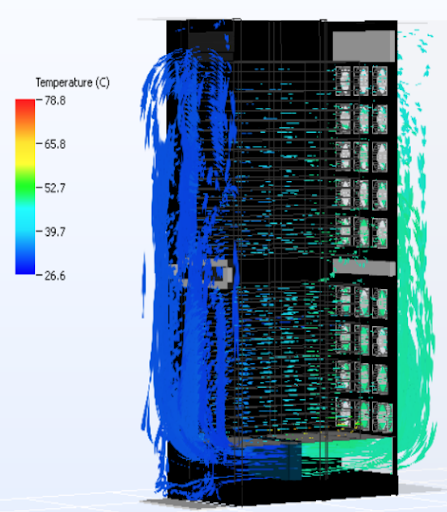
\includegraphics[width=0.4\textwidth]{methodology/images/bcu_rack.png}
        \label{bcu_rack}}
    \caption[Development of Bottom Cooling Units]{Development of Bottom Cooling Units. Image from \cite{gao16}}
\end{figure}
    
    The second order trade offs for such system include the changes required to the building systems, the impacts to the network topology, chiller plant augments, and power distribution. These trade-offs must be made with awareness of the data center service level agreements as not to strand space, power, or network ports. Furthermore, the business evaluation of such a development efforts must normalize all of the above factors to indicate cost vs. performance to allow consideration of alternate technologies as shown in Figure~\ref{img_bcu_second_order}.
    
    \begin{figure} [!h]
\centering
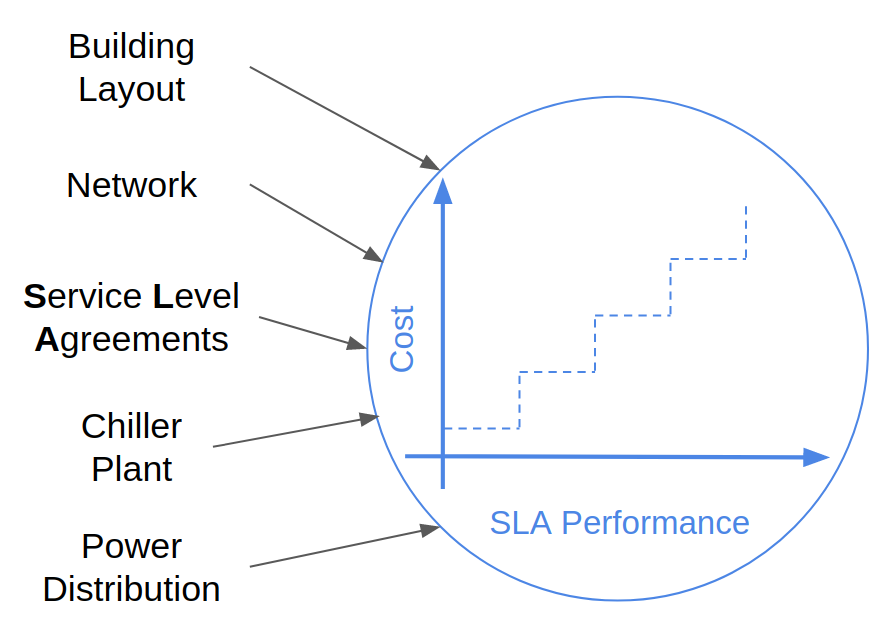
\includegraphics[scale=.25]{methodology/images/bcu_second_order.png}
\caption[Bottom Cooled Unit Second Order Trade-Offs]{Second Order Trade-offs.}
\label{img_bcu_second_order}
\end{figure}
    
    Beyond the operations phase of DCs, the IT hardware and physical infrastructure products they're composed of have many other life-cycle phases. At each life cycle phase of the products there are energy and $CO_2$ inventories. With life cycle analysis (LCA) principles these inventories can be tallied from their raw form to their useful state.  The LCA perspective allows the treatment of these inventories as either a debt or credit to it's environmental footprint. The debt and credit approach follows a structure analogous to total costs of ownership (TCO) methods used in today's sophisticated business models for DCs. These modern business models amortize capital and operating costs over a system's useful life similar to LCA. This research therefore threats $CO_2$ as analogous to monetary cost and demonstrates the end to end $CO_2$ inventories in this dissertation.
    
    The direct effects described so far and discussed throughout this work are the most transparent impacts associated with information communication technology (ICT). The indirect or higher order impacts fundamentally alter the use of energy in a wide breadth of applications. Figure~\ref{ICT_econ} shows examples of the breadth ICT impacts to other industrial sectors. However, this research followed the approach set by The Green Grid where the DC is a physical entity of interest and focuses on the assessment of it's direct life cycle activities \cite{tgg12}. The direct activities are indicated by the red boundary shown in figure  \ref{fig:f2} which sets the boundary conditions described later. 
    
    
\begin{figure}[!tbp]
    \subfloat[Influence and Impacts of ICT to other sectors]{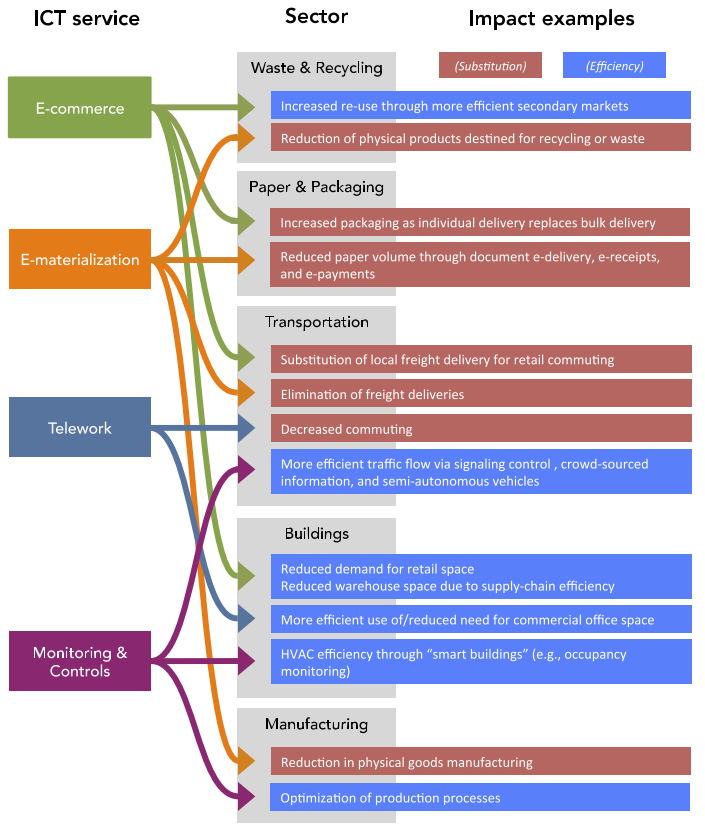
\includegraphics[width=0.5\textwidth]{methodology/images/ICT_econsec.png}
        \label{ICT_econ}}
    \hfill
    \subfloat[Taxonomy of ICT impacts]{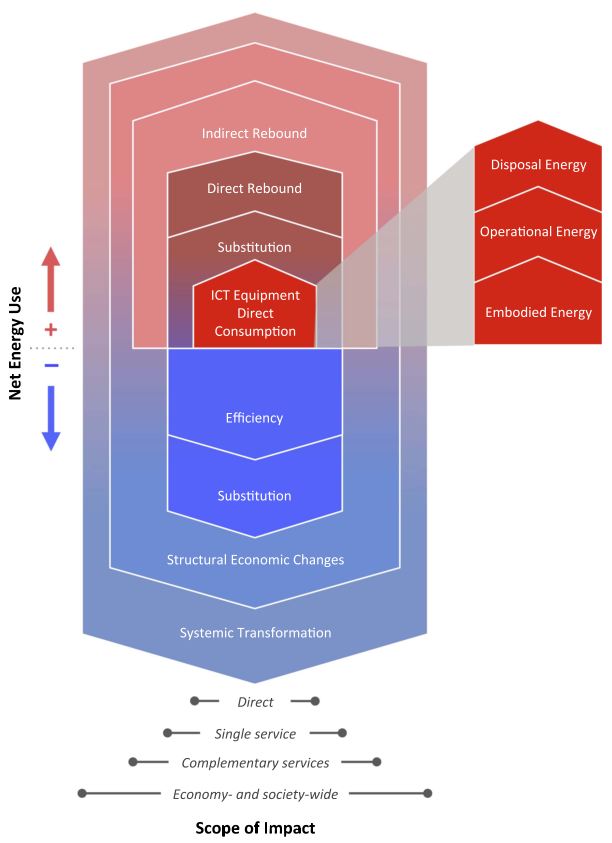
\includegraphics[width=0.4\textwidth]{methodology/images/ICT_scopes.png}
        \label{fig:f2}}
    \caption[Higher Order ICT Impacts]{Higher Order ICT Impacts. Images from \cite{Horner16b}}
\end{figure}
    
\section{Similar Works}
    
    Now, pioneering works that have quantified the life cycle costs of DCs are presented. The most explicit DC life cycle costs is by Whitehead \cite{whitehead15}. Whitehead proposes guidelines and criterion for DC life cycle assessments in-line with ISO 14040 \cite{ISO14040}. These ISO standards are the authoritative standard for Life Cycle Assessment (LCA) work.  Whitehead's work is based on the LCA of a UK DC with legacy infrastructure. The UK DC is compared to a state of the art DC in Sweden across all phases of their life cycle. The boundary conditions and life cycle phases from Whitehead are shown in figure \ref{LCAphases}. Through sensitivity analysis, Whitehead finds that server stock turnover (refresh) cycles have  the most significant contribution to the embodied impacts in today's state of the art DCs.  Embodied impacts for these DCs dominate the life cycle impacts even more so as the state of the art DCs are optimized for PUE with efficient cooling and power distribution systems . To demonstrate, they performed a comparative evaluation. When quantified, the environmental impacts were double for the Swedish facility. Whitehead attributes this difference to the Swedish data refresh cycle of every 16 months, as opposed to every 36 months for the UK DC. They establish a functional unit of \textit{1 kW of IT per year in a Tier III facility} which is a reasonable units of measure of data centers.
    
    \begin{figure} [!h]
\centering
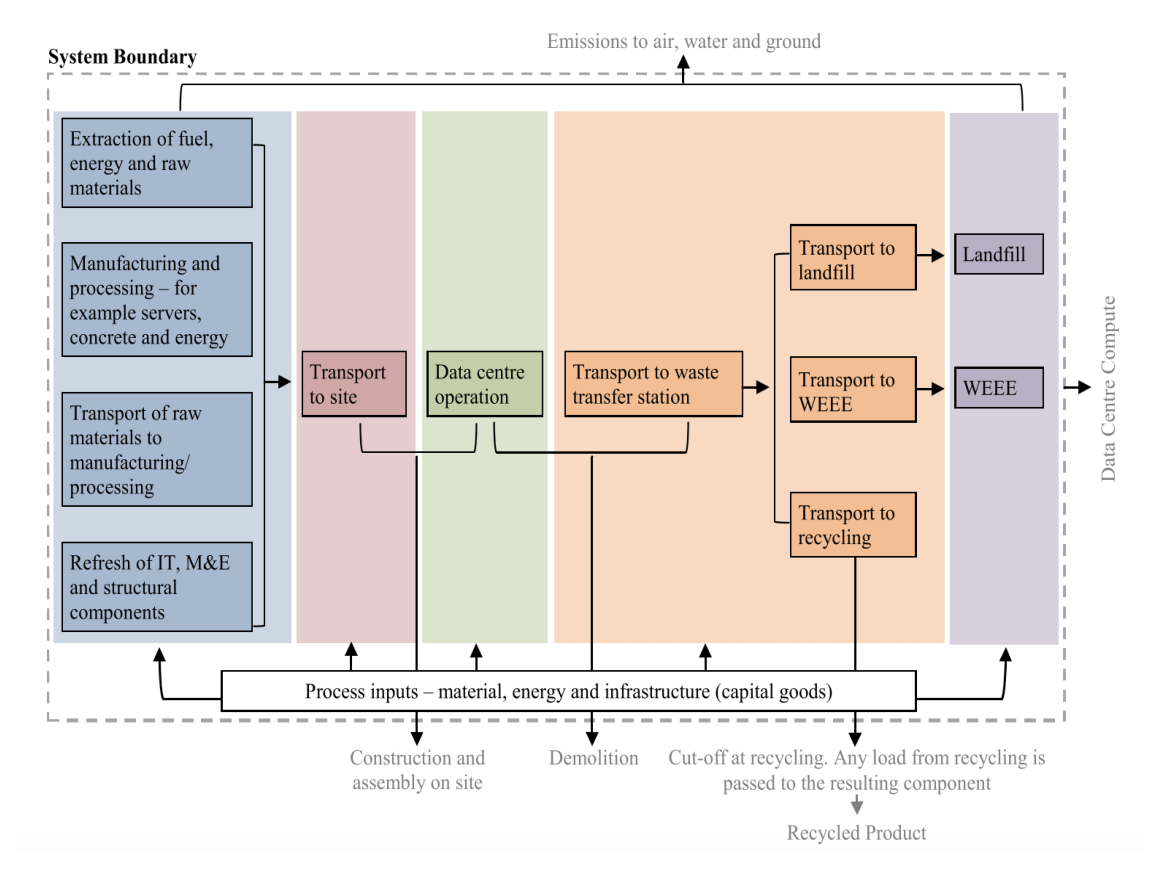
\includegraphics[scale=.6]{methodology/images/LCAphases.eps}
\caption[Whitehead DC LCA Boundary]{System boundary for DCs. Image from \cite{whitehead15}}
\label{LCAphases}
\end{figure}
    
    The Hewlett Packard Corporation published a series of papers around the sustainability of information technology sector in the early 2010's. Two of the most relevant to data centers were led by Shah and Chang \cite{shah11, shah12}. In the first work, Shah demonstrated the use of the economic input-output (EIO) model for assessing the embodied costs of the major infrastructure categories found in data-centers (see Table \ref{shah_components}). Their development of the environmental model for the data center was ultimately a combination of process based and EIO methods. Building on Shahs's EIO based framework, Chang uses the thermodynamic metric of exergy to quantify data center sustainability. By quantifying the irreversible thermodynamic processes in terms of exergy allows normalization in terms of architectural parameters \cite{shah12}. A parametric view enables systems designers to reason about only an intuitive set of constraints.
    
    \begin{table}[h!]
    \begin{center}
    \scalebox{0.6}{
    \pgfplotstabletypeset[
        col sep=comma,
        string type,
        every head row/.style={before row=\hline,after row=\hline\hline},
        every last row/.style={after row=\hline},
        ]{methodology/content/data/shah_boundaries.csv}}
    \end{center}
    \caption{Components considered by Shah \cite{shah11}
}    \label{shah_components}
\end{table}

    
    In addition to the independent LCA perspective of Whitehead and the corporate perspective of Hewlett Packard, The Department of Energy's Lawrence Berkeley National Lab  has produced the CLEER online modeling tool\cite{CLEER13}. CLEER is a web based user interface that allows consumers to model the migration of the CLEER model to assess the life cycle cost of migrating on-premise software workloads to Cloud based data center platforms. As shown in Figure~\ref{img_cleer}, the charter for the CLEER model to consider the end to end energy associated with Cloud services.
    
    \begin{figure} [!h]
\centering
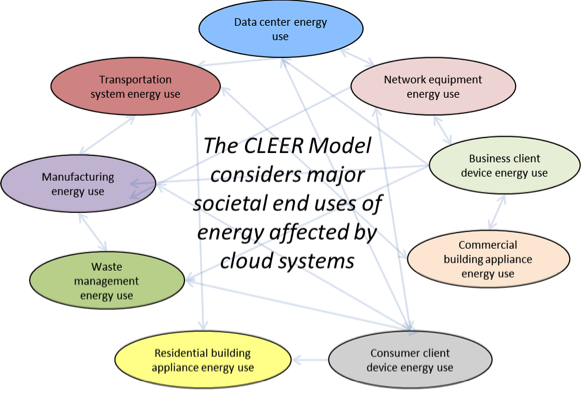
\includegraphics[scale=.5]{methodology/images/cleer_diagram.png}
\caption[CLEER Framework]{CLEER Framework.  Image from \cite{CLEER13}}
\label{img_cleer}
\end{figure}
    
    In the subsequent chapters, this research builds upon these pioneering similar works. Six parameters common to all three are identified and supplemented with novel contributions developed by this dissertations research. Two additional are also added to make the end to end modeling framework presented dynamic in terms of network traffic and building operations as shown in Figure~\ref{img_gap_matrix}
    
    \begin{figure} [!h]
\centering
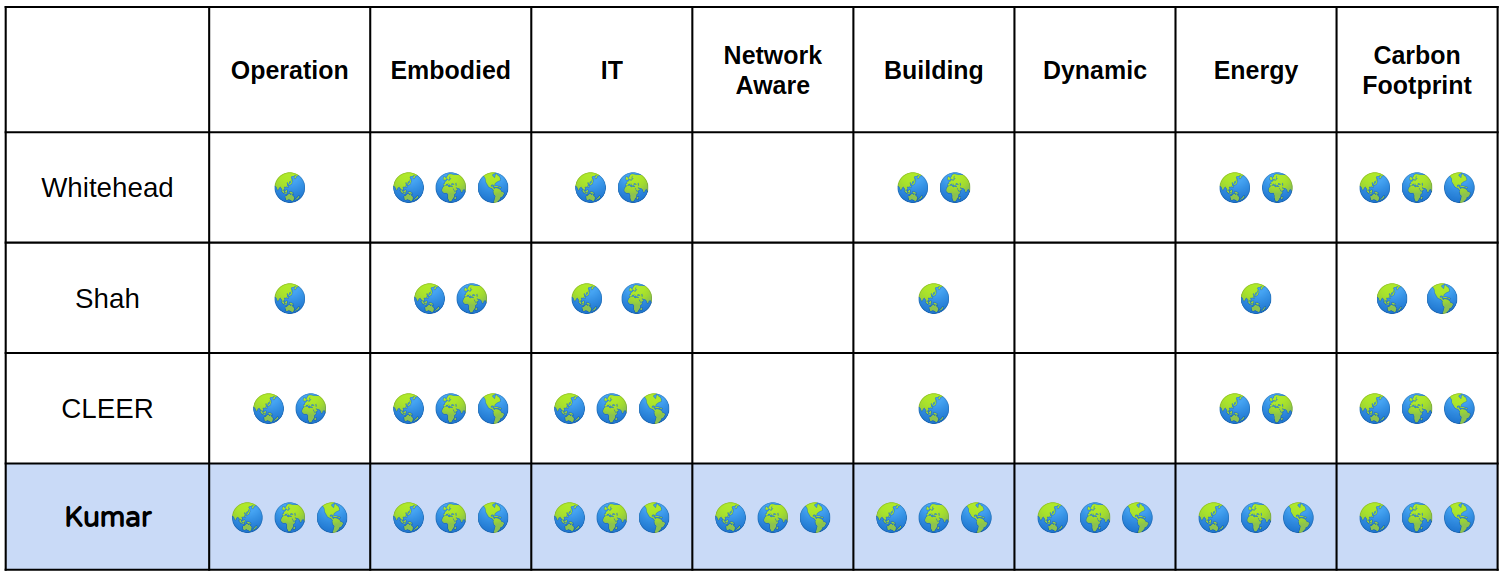
\includegraphics[scale=.25]{methodology/images/gap_matrix.png}
\caption[Research Gap Matrix]{Gap Matrix.}
\label{img_gap_matrix}
\end{figure}
    
    The background discussed in this section inspires the research question pursued through the dissertation. Namely the research question is \emph{how can DC designers make decisions that have longevity with all of the uncertainty involved?} Next the research hypothesis is stated followed by and overview of the specific methods that are used to validate the hypothesis.
    
\section{Hypothesis}

    \emph{\large To make effective DC design capacity decisions, the decisions must be based on scalable and agile models.}
        
    Sub hypothesis are as follows:
    
    \begin{enumerate}
        \item The model needs to assess end to end cost trade-offs and be technology agnostic.
    
        \item Monetary cost models for DCs are analogous to environmental cost models. LCA modeling community has proven its effectiveness for analysing global scale systems and supply chains.
    \end{enumerate}
    
\section{Structure of Dissertation}

    This research is composed of four modules that culminate academic desktop analysis and extensive professional experience with designing, planning, building, and deploying data center system through out the world. The modules are presented in this dissertation as independent, but correlated chapters. The segmentation of the chapters roughly aligns with the software modules developed as shown in Figure~\ref{process_flow}.
    
    \begin{figure}[h]
\centering
\begin{tikzpicture}
\node [anchor=west] (scope) at (8.75,5.5) {Embodied Costs};
\node [anchor=west] (traffic) at (1.4,5.5) {Traffic};
\node [anchor=west] (bem) at (4.2,5.5) {BEM};
\node [anchor=west] (mec) at (6.75,5.5) {MEC};
\begin{scope}[xshift=1.5cm]
    \node[anchor=south west,inner sep=0] (image) at (0,0) {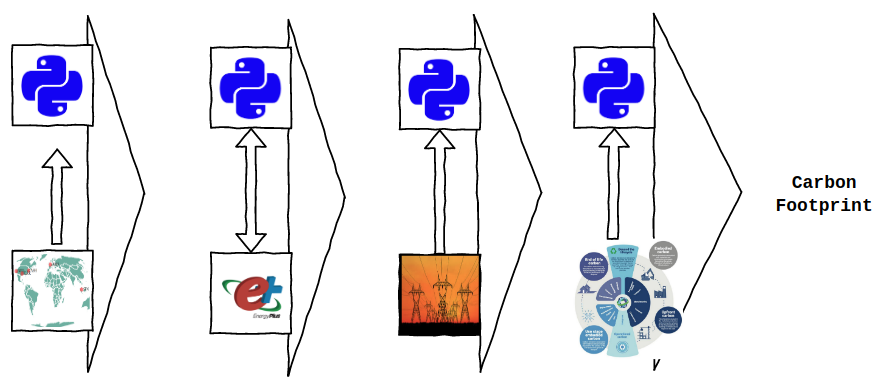
\includegraphics[width=0.8\textwidth]{embodied_cost_model/images/horizontal_process_flow.png}};
    \begin{scope}[x={(image.south east)},y={(image.north west)}]
        % \draw[ultra thick,rounded corners, ,dashed] (0.625,1.0) rectangle (0.85,0.0);
        % \draw [-stealth, line width=5pt, cyan] (scope) -- ++(0.6,0.0);
    \end{scope}
\end{scope}
\end{tikzpicture}
\caption[Model Process Flow Diagram]{Model Process Flow Diagram.}
\label{process_flow}
\end{figure}

\section{Overview of Data Center Systems.}
    The research's understanding of data centers and the various systems with-in data centers are now presented. The first systems addressed are the information technology equipment. The information technology equipment have two points of significance in the overall research objective. First, a detailed bill of materials of all the equipment is required to quantify the embodied energy. Second, in the operational phase each piece of information technology device has a unique power use profile. Therefore, ensemble representations of servers without the consideration of the individual components that only provide coarse insights of both embodied and operational energy may not be generalized across different data centers. 
    
    The second set of systems addressed are data center communication networks. The network is a critical component that is at the core of hyper-scale data centers. Its the network that allows data center services to appear to its users as a single coherent system whether they are located in the same rack are globally dispersed \cite{steen17}.
    
    The third system addressed in this section are the building systems. The building systems are the key focus of this research and this section aims to identify the key parameters that make data center facilities distinguishable from other building types. 
    
    The underlying data sources that construct and validate the developed software modules are sourced from publicly available references and professional heuristics. Generally, the preference of this research is to use publicly available data for academic posterity, however there are several critical pieces of information that can not be publicly disclosed. In these cases, where no relevant public information was found, the author leans on professional heuristics. 
    
    Due to the nature of the technology business, most of the heuristically derived data points are protected under non-disclosure agreements. Every effort is made not to impede these agreements.
    
    The following subsections provide overviews of the information technology equipment, communications networks, and buildings as they are reasoned about in this research.
    
        \subsubsection{Information Technology Equipment (IT)}
            The modeling framework developed in this research is founded upon the information technology hardware housed inside data centers. Table~\ref{computer_parts} indicates the data used in this research to characterize the information technology hardware that are inputs to building energy simulations and embodied materials models. There server profiles are based on production server configurations of a large internet operator, representing their deployments in 2015 and 2016. However, the objective of the research is to have the agility to model any allocation of individual components found in data centers. Some of the current approaches for allocating servers and their components are described next.
            
            Servers are generally categorized as compute nodes or storage nodes. Compute servers maybe fitted with state-of-the-art processors, input and output devices, and dynamic random access memory (DRAM). The latter category of storage servers are optimized for high density storage with minimal processor capabilities with input output devices selected based on the desired performance. Figure~\ref{img_server} shows air cooled server units fitted with a combination of processors and DRAM. While Figure~\ref{img_storage_tray} shows a homogeneous arrangement of storage drives in a server. 
             \begin{figure} [!h]
\centering
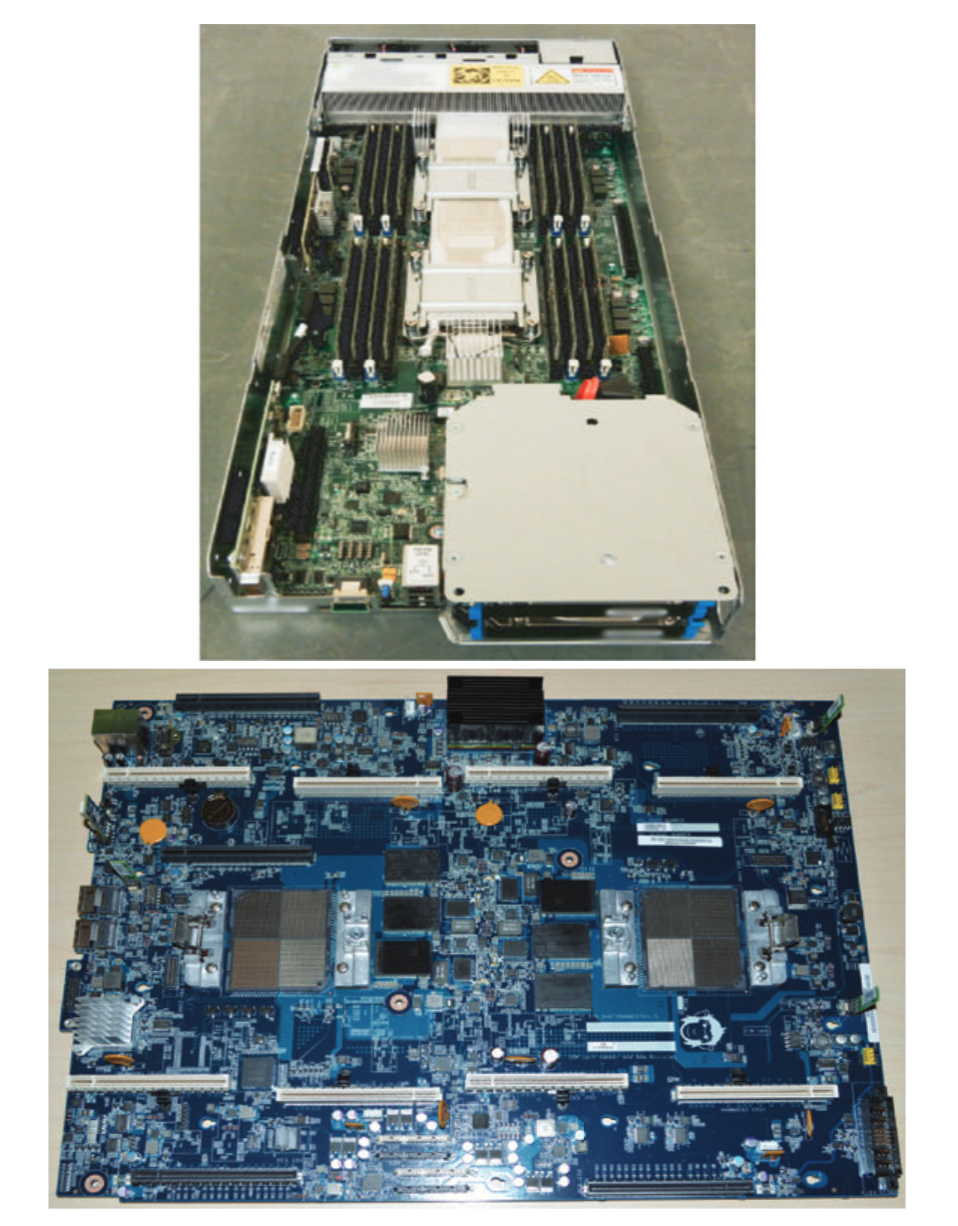
\includegraphics[scale=.5]{methodology/images/server_image.png}
\caption[Barroso's Servers]{(Top) Intel Haswell-based server tray and (Bottom) IBM Pow-er8-based server tray.  Images from \cite{barroso13}}
\label{img_server}
\end{figure}
            \begin{figure} [!h]
\centering
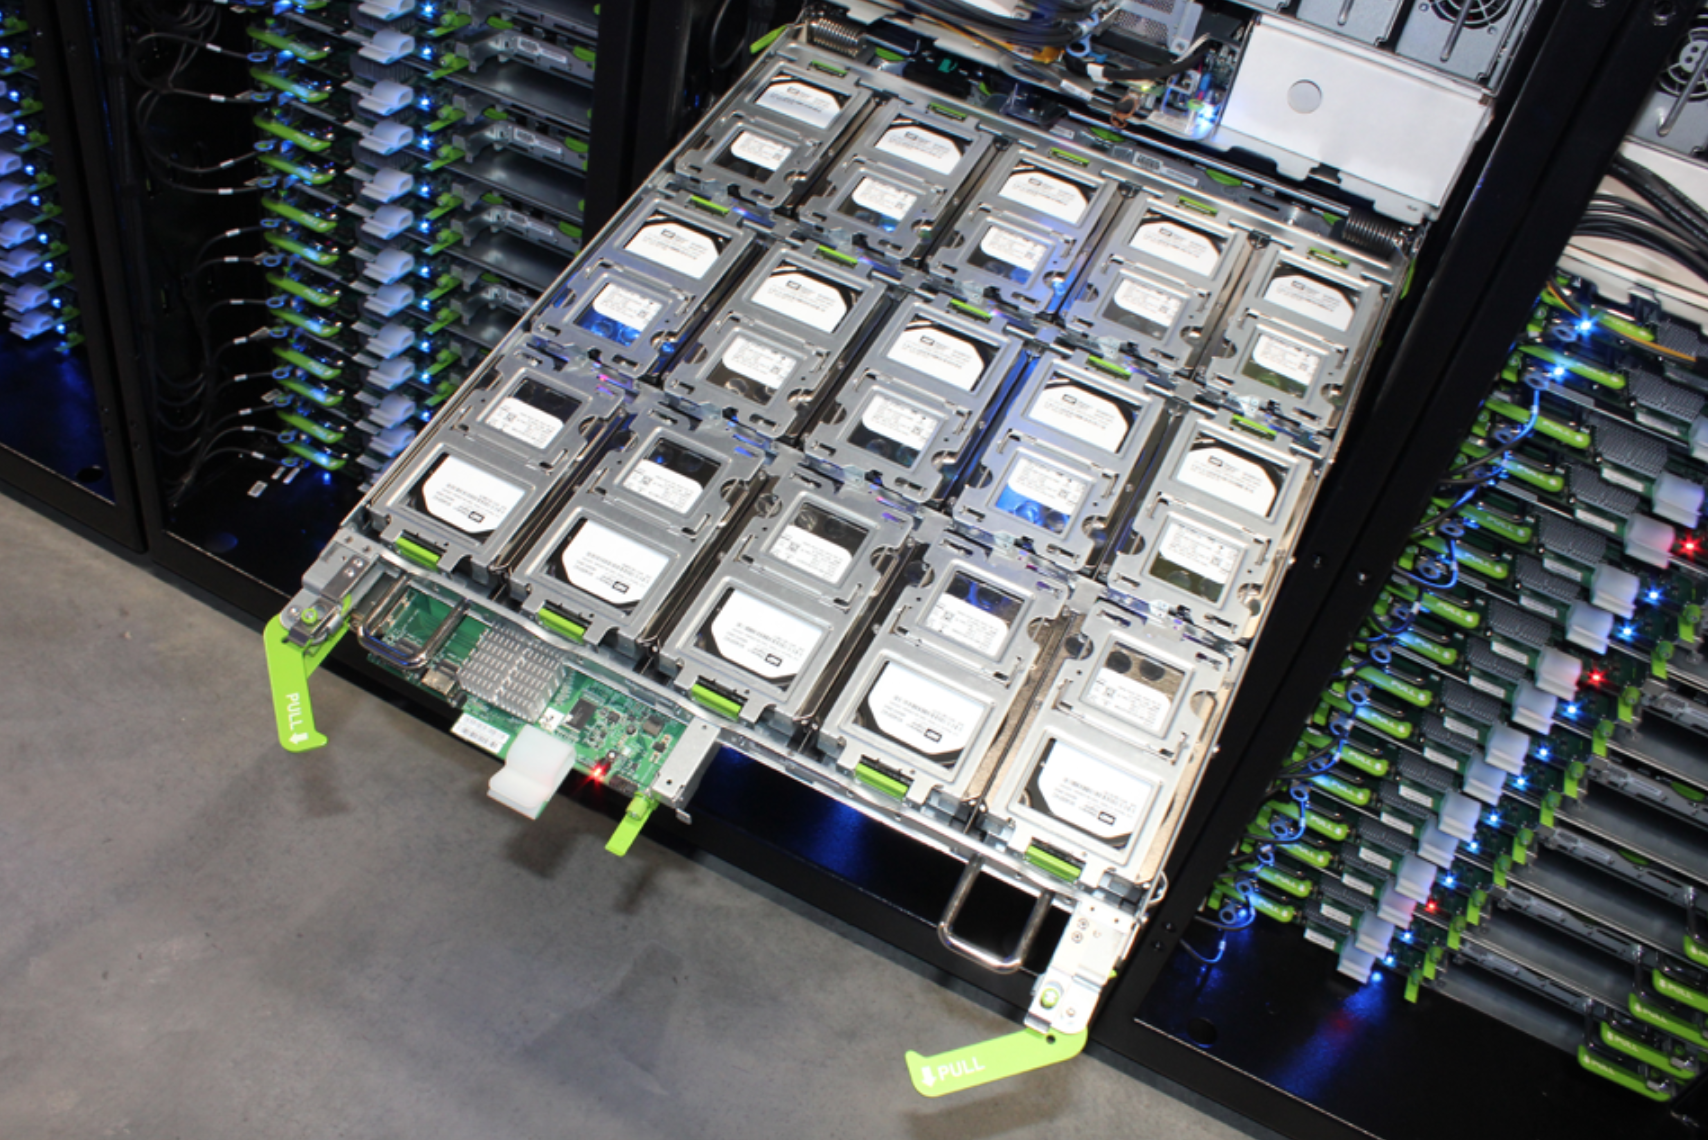
\includegraphics[scale=.3]{methodology/images/storage_tray.png}
\caption[Storage Servers]{Storage Servers - Homogeneous Storage Server Tray.  Image from \cite{cisco_storage}}
\label{img_storage_tray}
\end{figure}
            
            Segregating the storage from the compute instances have several advantage for the software architecture; for building systems designers the most intuitive is failure isolation and operational diversity. For consideration of failure isolation, the outage of a single compute instance will also result in the stored data becoming unavailable. In terms of diversity, when compute devices and storage devices are on the same physical equipment the single processing device may not be capable of handling the all the requests to access the stored data within performance bounds. Separating the data into different servers allows the incoming read or write requests for the stored data to be balanced across a set of processors based on performance bounds. This relationships is the premise of many modern data center cluster designs, where stored data and compute resources are strategically arranged. Figure~\ref{img_cluster_storage_hierarchy} indicates such a cluster storage hierarchical scheme from Barroso \cite{barroso18}. 
            
            \begin{figure} [!h]
\centering
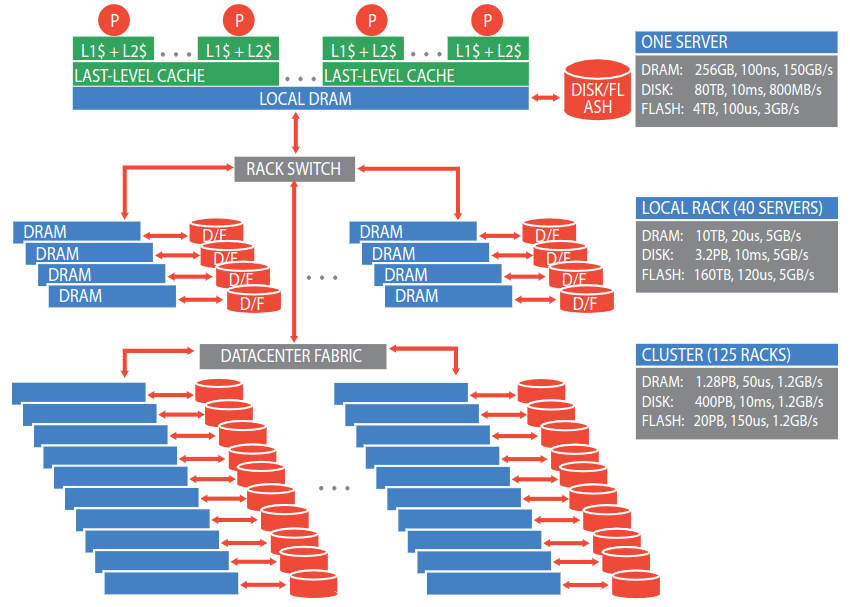
\includegraphics[scale=.35]{methodology/images/cluster_storage_hierarchy.png}
\caption[Cluster Storage Hierarchy]{Storage hierarchy of a warehouse scale computer. The concept of a cluster loosely follows this topology. Image from \cite{barroso18}}
\label{img_cluster_storage_hierarchy}
\end{figure}
            
            In this work, a combination of compute and storage components are aggregated for modeling as listed Table~\ref{computer_parts}. The power demand for these components are noted in Table~\ref{tab:it_component_power_dist_table}. The combination of component counts and power allows for the the total power of the servers to be quantified. In the servers studied, their total power demand range from 320 watts to 332 watts.  These heterogeneous server choices suffice for this dissertation because of two reasons. (1) research had first hand access to representative cost data for these servers. (2) mixed component server assemblies can properly characterize the embodied materials of the overall data center. Nonetheless, the model developed is extensible towards other server component mixes. 
             \begin{table}[h!]
    \begin{center}
    \scalebox{0.5}{
    \pgfplotstabletypeset[
        col sep=comma,
        string type,
        every head row/.style={before row=\hline,after row=\hline\hline},
        every last row/.style={after row=\hline},
        ]{methodology/content/data/Server_Component_Counts.csv}}
    \end{center}
    \caption[Server types and components used in modeling]{Server types and components within these servers modeled in the simulations performed for this research.}
    \label{computer_parts}
\end{table}
            
            Furthermore, the mixed component servers lend themselves to simplified allocation of various components within the data center building and allow for non-linear scaling of the various components. This simplification enabled by the mixed server types allows the quantification of the component counts using the top down relationship to the total power of the building using Algorithm~ \ref{it_y_vector_algo}. This is sufficient for building design tasks as it captures all of the components that influence life cycle cost models. Finer granularity is not sought as the models that are developed in this research don't optimize or even account for the air flow patterns or equipment layout inside the buildings. Nonetheless the accuracy of the framework can be enhanced for quantifying the operational energy and embodied materials if the physical layouts of the servers are more precisely characterised in future work. Next, racks that host the server chassis are discussed.
            
            %  Examples of the design choices for the server components arrangements and building layouts are now discussed. These examples point to modeling improvements that can make this framework more precise. Furthermore, these example are used to normalize the servers into their deploy-able units; a server rack.
            
            Steel racks host the server assemblies. Figure~\ref{bcu_rack} and Figure~\ref{goog_rack} are examples of racks found inside warehouse-scale data centers. At the rack level, the servers can be mixed and matched with a high speed hermetic network within the rack (see Figure~\ref{img_server_rack}. Alternately, the entire rack can be of a single type, bridged by high speed communications networks across local areas that connect racks dispersed within the  latency bounds set by the communication optical instruments and cables as  discussed in the Network part of subsection~\ref{Network}. 
            
            The choice for the rack arrangement is reasoned about as performance objectives for specific workloads that the rack will be susceptible to. In the end whether at a the individual server, rack level, or cluster level; compute and storage devices need to communicate with each other as shown in Figure~\ref{img_cluster_storage_hierarchy}. Specific design choices must optimize the service level performance objective in terms of the attributes noted in Figure~\ref{img_cluster_storage_hierarchy} namely data volume, read/write latency, and the read/write rates.
            
            \begin{figure} [!h]
\centering
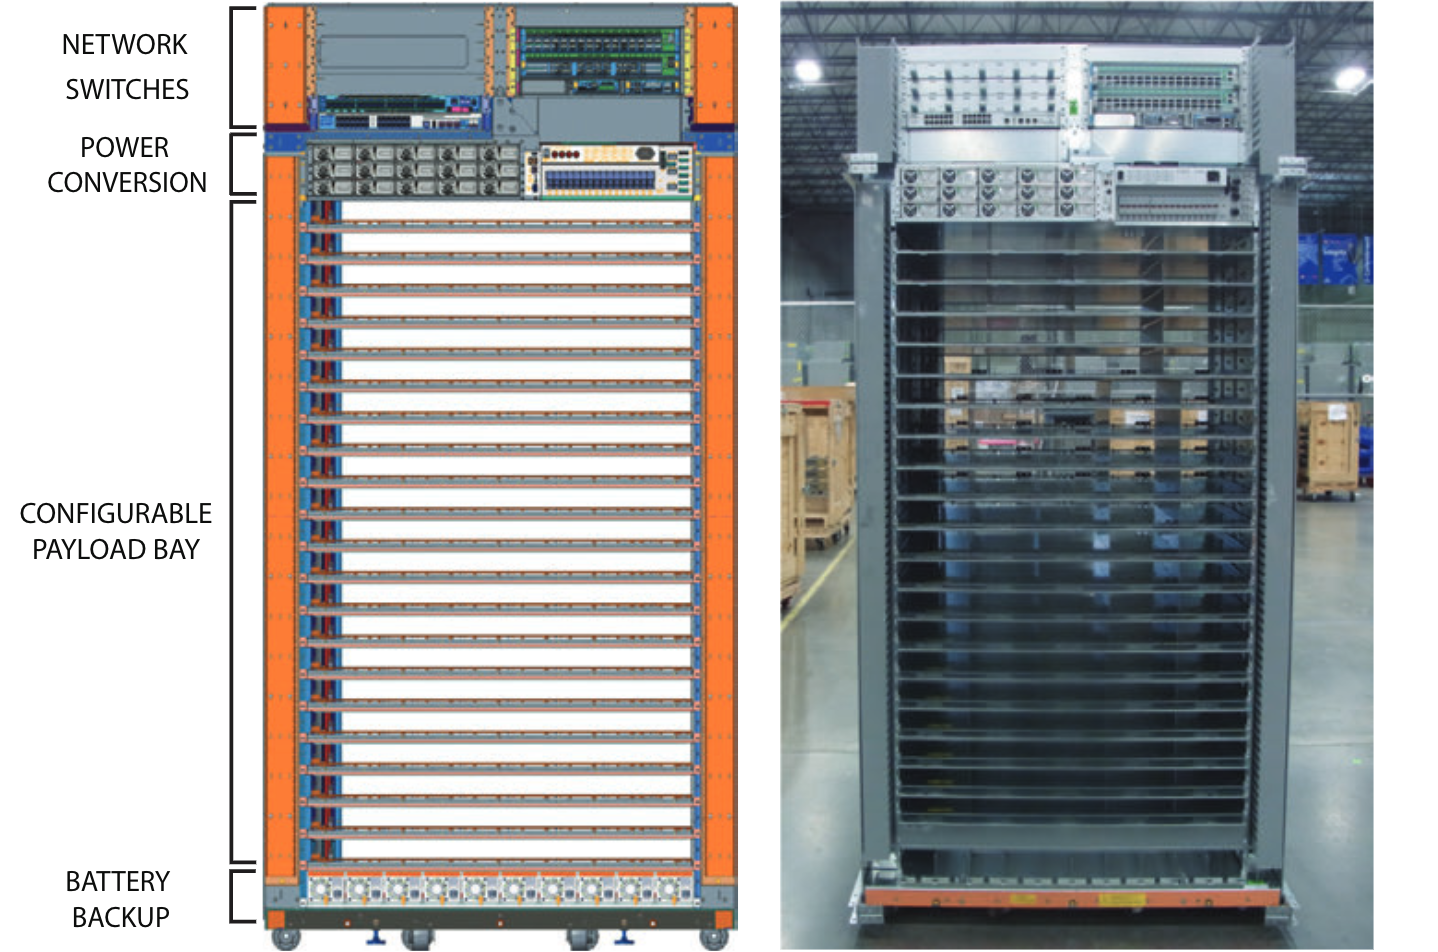
\includegraphics[scale=.5]{methodology/images/goog_rack.png}
\caption[Example Server Rack]{Server rack with top of rack switch, power shelf, server trays slots, and local batteries. Image from \cite{barroso18}}
\label{goog_rack}
\end{figure}
            
            As shown in Figure~\ref{goog_rack}, a server rack hosts local power conditioning, power distribution, and network devices as-well. The incoming power feed is generally AC voltage where as all the server components require DC voltage. In legacy servers the AC to DC voltage conversion happened within the server, however in modern racks the power is rectified at the rack level with more efficient rectifiers and distributed with 48V bus bars \cite{open_compute_48V}. The rectification leads to some additional heat at the rack level in addition to the server heat. Also at the rack level, there exist the network devices, commonly termed top of rack (TOR) switches. These TORs are a hub for all the server's communications cables. The network connections are discussed next. 
    
        \subsubsection{Network Model}
        \label{Network}
        A generic server rack arrangement and the network connections relative to the rack is indicated in \ref{img_server_rack}. The servers can communicate with other collocated servers in the rack up to the full bandwidth allowed by their network cards. This is sufficient for many services and is a reason to mix storage and CPU servers at the rack level. However in large distributed systems, it is not trivial to provision a static dependencies between processes and stored data (a couple challenges are noted above). 
    
        \begin{figure} [!h]
\centering
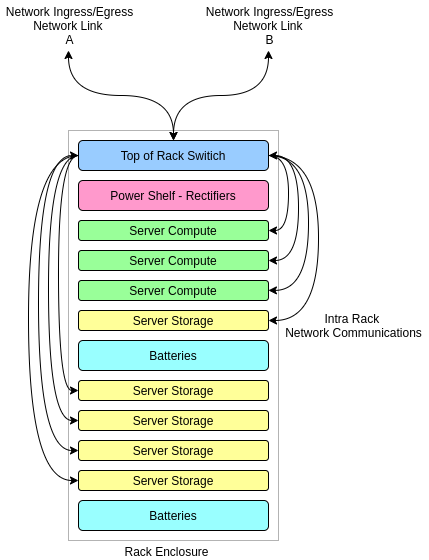
\includegraphics[scale=.5]{methodology/images/Server Rack.png}
\caption[Server Rack Communications Network]{Server Rack Communications Network}
\label{img_server_rack}
\end{figure}
        
        When processing servers and storage servers are not collocated on a rack, they must be bridged together with high speed communication networks. A collection of densely connected servers over a communication network is a cluster. A popular network topology with in clusters is illustrated in Figure~\ref{img_fb_clos}. The physical layout of the cluster is limited by the fiber optics and cable. The distance limits for multimode fiber cables used inside DCs are indicated in Table~\ref{table_fiber_limits}.
        
        \begin{figure} [!h]
\centering
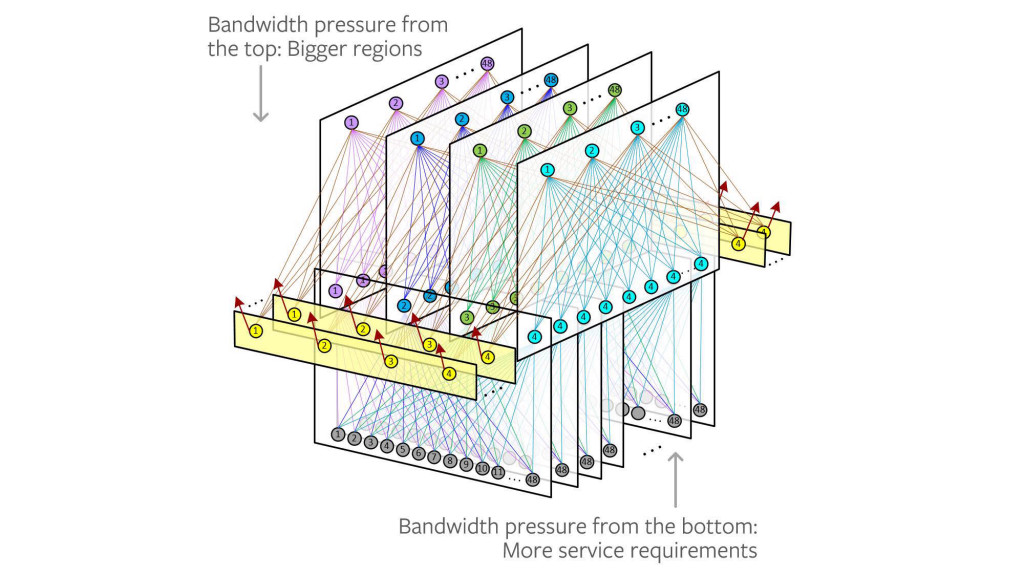
\includegraphics[scale=6]{methodology/images/fb_clos.jpg}
\caption[DC Clos Network]{Data Center Clos Cluster Network Mesh. The surface planes running upward from left to right has two layers of 4-post (3+1 redundancy) rack TOR aggregation nodes in each surface. The bottom most nodes on the surface planes running downward from left to right, capture the server rack nodes. Each rack connects to all four posts of the aggregation layers.  Image from  \cite{fb_clos}.}
\label{img_fb_clos}
\end{figure}
        
        \begin{table}[h!]
    \begin{center}
    \scalebox{0.7}{
    \pgfplotstabletypeset[
        col sep=comma,
        string type,
        every head row/.style={before row=\hline,after row=\hline\hline},
        every last row/.style={after row=\hline},
        ]{methodology/content/data/fiber_limitations.csv}}
    \end{center}
    \caption[Fiber Limits]{Communication capacity distance limitations. Data sourced from \cite{cleerline}.}
    \label{table_fiber_limits}
\end{table}
        
        \subsubsection{Building Systems}
        
        The form factor of data center facilities are heavily influenced by the mechanical systems conveying heat from the racks a heat sink. Figure~\ref{img_airflow} illustrates the airflow path across a data center from the point that air enters the building until it is exhausted. A server room layout is also heavily guided by the the mechanical cooling systems. Figure~\ref{img_server_room} illustrates a room layout with arrays contiguous server rows. The air space between the servers are segregated for either hot or cold air, where the front of the servers are in the cold aisle and the back of the servers are in the hot air aisles. 
        
        \begin{figure} [!h]
\centering
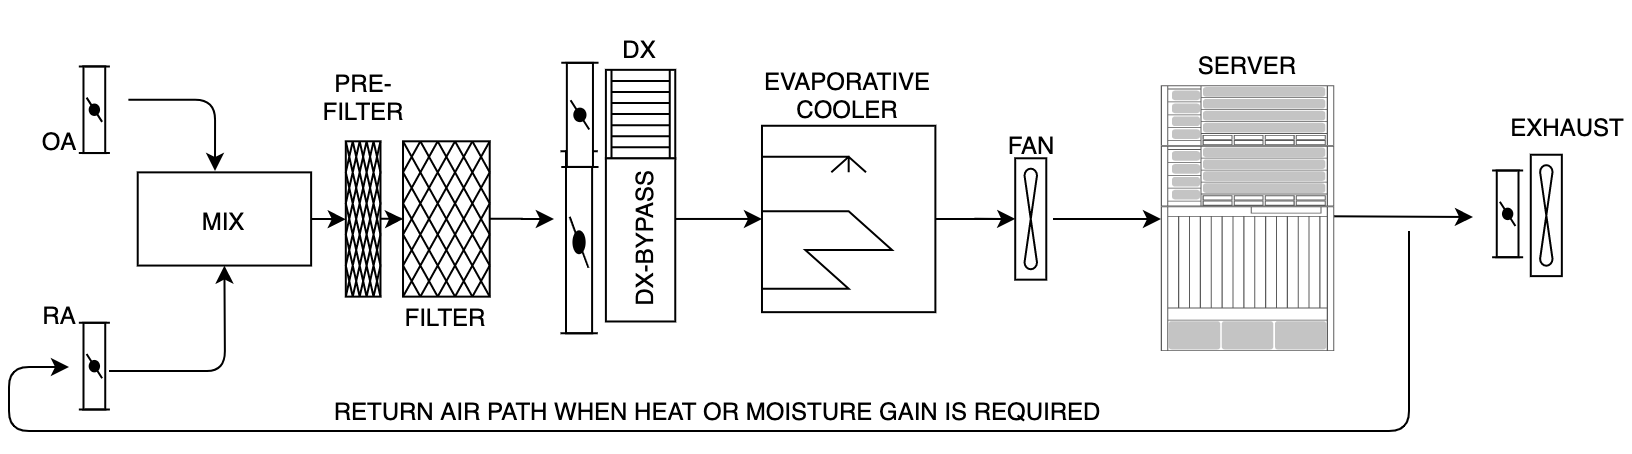
\includegraphics[scale=.5]{methodology/images/airflow.png}
\caption[Airflow through DCS]{Generic air flow path in server rooms for an outside air cooled facility.}
\label{img_airflow}
\end{figure}
        \begin{figure} [!h]
\centering
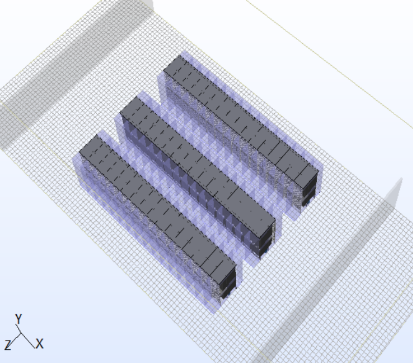
\includegraphics[scale=.5]{methodology/images/server_room.png}

\caption[Server room layout]{Server room layout. The gray elements in the figure are the hot aisles and the light purple elements are the server racks. The objective of the cited work was to determine the optimal spacing of adjacent racks across hot-aisles.  Image from \cite{sahini16}}
\label{img_server_room}
\end{figure}
        
        The building attributes that guide this research are obtained from real world hyper-scale designs and their construction costs in various regions around the world. Specific building designs are not be explicitly disclosed in this dissertation and the costs data have been normalized across the set of real world examples per kW of provision-able capacity at the respective data center. The most influential data center attribute, the power density, ranged from 1.99kW per meter squared to 3.3kW meter square. Next the above systems are tied back to spatial area of the data centers; namely the rack form-factor. 
        
        \begin{table}[h!]
    \begin{center}
    \scalebox{0.5}{
    \pgfplotstabletypeset[
        col sep=comma,
        string type,
        every head row/.style={before row=\hline,after row=\hline\hline},
        every last row/.style={after row=\hline},
        ]{methodology/content/data/building_costs.csv}}
    \end{center}
    \caption{Relative Costs of Sub Components and DC Building
}    \label{table_building_costs}
\end{table}
        
    \section{Tieing it all back to deployable increments of IT equipment}
    
    Hyperscale data centers are often populated on an incremental basis. The deployment increments are typically in the form-factor of a rack. The rack level deployment provides a clear interface with the building systems. For example when the racks are independent failure domains, it can be easily isolated with a dedicated electrical breaker at this level. Also, a fully populated rack is much easier to reason about for capacity constraints from a power and cooling standpoint. 
    
    Capacity constraint management is a critical part of data center operations, as IT devices can be added, removed, and replaced at any time during the life of the facility. Deployment of partially populated racks risks capacity being stranded or over subscription of resources (i.e. head room on the electrical breaker) if the end states of all deployable rack positions are not sequentially deterministic. To reclaim the stranded power racks requires re-shuffling of racks across a data center to de-fragment the floor space. While, over-subscription is handled by physically moving racks as-well. The cost of rack moves includes the down time of a rack and staffing/engineering toil and is handled with resistance in practice.
    
    In the models developed for this research, for simplicity and its purpose as a proof of concept framework, the deployment increments are not considered. The information technology considerations of this research are indicated in Table~\ref{computer_parts}. These components are bin packed into the power envelope per Algorithm~\ref{it_y_vector_algo} to quantify the input costs for the EIO. This level of aggregation may suffice for monolithic clusters, but it may not work for highly diverse workloads (like public cloud operations). To translate the components into the count of deploy-able racks, requires additional insights about the server rack layouts in relationship to the rest of the building floor area. The equation presents the methods to translate the server power density to rack counts and rack level power.
    
        \begin{equation} 
    \label{eq:floor_per_density}
        \rho= \frac{P_{f}}{A_{F}}
    \end{equation}
    
    \begin{equation} 
    \label{eq:area_for_racks}
        A_{r}= A_{f} \times F_{f}
    \end{equation}
    
    \begin{equation} 
    \label{eq:rack_count}
        R_{\#}= \frac{A_{r}}{R_{a}}
    \end{equation}
    
    \begin{equation} 
    \label{eq:rack_power_server}
        P_rs = \frac{P_f \times (1-F_{n})}{R_{\#}}
    \end{equation} 
    
    \begin{equation} 
    \label{eq:rack_power_network}   
        P_rn = P_rs \times F_{n}
    \end{equation} 
     
    \begin{equation} 
    \label{eq:rack_power} 
        P_r = P_{rs} + P_{rn}
    \end{equation} 
    
    \begin{small}
    \begin{center}
    
    $\rho$ = Power Density of server floor. This value is used in the EnergyPlus Models.
    
    $A_{f}$ = Total floor area
    
    $A_{r}$ = Area available for rack deployment
    
    $R_{a}$ = Rack footprint area
    
    $R_{\#}$ = Rack count
    
    $P_{f}$ = Provisioned power for IT for server floor.
    
    $P_{rs}$ = Power for rack server equipment.
    
    $P_{rn}$ = Power for rack network equipment.
    
    $P_{r}$ = Total power of rack.
    
    $F_{f}$ = Fraction of $A_{f}$ that is deploy able with Racks.
    
    $F_{n}$ = Fraction of power to rack allocated to network devices. 
    
    \end{center}
    \end{small}
    
    Equation~\ref{eq:floor_per_density} indicates the  IT load density that is input to each thermal zone. However, this density is a naive distribution of the IT load over the entire floor area; while servers can only be positioned in linear rows as shown in Figure \ref{img_server_room}. This rack layout reduces the area available for racks. Equation~\ref{eq:area_for_racks} accounts for the fraction of the server floor where racks can be deployed. Once the area for racks is known, the quantity of racks that the server floor can support can be evaluated with Equation \ref{eq:rack_count} and the average power for each rack can be evaluated with Equation \ref{eq:rack_power}.
    
    By using the above equations, the rack power derivation from known values on power capacity and building layouts is shown in Table~\ref{table_rack_power}. The calculations are based on a 7,500 kW data center. The building area, server rack form factors, and the network coefficients are input based on the specifications of this data center. As shown in the table, the average supportable rack power is 6.5 kW. Above the power demands ranges from 320 Watts to 332 Watts for each of the servers in the research's data set, each rack can support 20-21 servers.
    
    \begin{table}[h!]
    \begin{center}
    \scalebox{0.7}{
    \pgfplotstabletypeset[
        col sep=comma,
        string type,
        every head row/.style={before row=\hline,after row=\hline\hline},
        every last row/.style={after row=\hline},
        ]{methodology/content/data/rack_power.csv}}
    \end{center}
    \caption[Example Rack Power]{Example of rack power for server floor power density values.}
    \label{table_rack_power}
\end{table}.
    
    There are several other constraints that must be optimized in real world data center deployments; for example, power phase balancing, network bandwidth, network ports, heat rejection rates, air flow rates, along with several other fluid mechanics considerations. Each of these must be addressed on a situational basis and is left to future work around this framework.
        
    
   
    

    
    
